\chapter{1988 - CYB i USA!}

\author{Av Morten Moen \& Ole Christian Lingjærde}

\section{Planlegging og reise}

Vårsemesteret 1988 satt Morten som styreleder i CYB. Slik han husker det var det på et improvisert styremøte i Sky-baren på toppen av det som den gangen var SAS-hotellet tidlig den vinteren at tanken om en USA-tur ble født. Vi visste at CYB hadde vært der før, og vi ville gjøre noe større og bedre.

Ole Christian og Morten hadde ansvaret for programmet i USA mens Ole Christian og Aina Hegdalsaunet sto for reise-arrangementene. Etter hvert ble reiseruta som følger:

\begin{itemize}
	\item Fly Oslo - New York og New York-Boston
	\item Besøk på Apollo Computer, Thinking Machines, MITs AI-Lab og Media-Lab, og Boston Computer Museum.
	\item Fly Boston - San Francisco
	\item Besøk på Sun Microsystems og Amdahl
	\item Bil-etappe San Francisco - Los Angeles
	\item Fly Los Angeles - Orlando
	\item Fly Orlando - New York - Oslo
\end{itemize}

Et hovedfokus for oss i planleggingen var Amdahl Computers. Dette firmaet som sluttet å eksistere i 1997 ble startet av Gene Amdahl og produserte store mainframe-maskiner. Hans foreldre hadde utvandret fra Norge og Sverige, så firmaet syntes det var stas å få besøk av norske studenter. Hos de andre firmaene vi besøkte hadde vi bare mail-kontakt, men hos Amdahl ble Ole Christian og jeg invitert på et møte på kontoret i Oslo. Det var tydelig at de syntes det var stas at vi var interesserte i firmaet deres.

Selve reise-planleggingen ble som sagt tatt hånd om av Ole Christian og Aina, og de gjorde en fantastisk jobb! Det snakkes om at å fly har blitt veldig billig nå, men det var også mulig å få rimelige billetter den gangen, Vi reiste med Tjæreborg tur\slash retur New York. Dette kostet totalt 4870 kroner. Det er kanskje ikke så vanvittig billig, men Tjæreborg hadde et opplegg med noe som het Cis-tours som var slik at hvis vi booket t\slash r med Tjæreborg fikk vi alle de andre flightene, dvs

\begin{itemize}
	\item New York - Boston
	\item Boston - San F
	\item Los Angeles - Orlando
	\item Orlando - New York
\end{itemize}

med Delta Air for \$75 og det må jo kalles relativt rimelig.

\begin{figure}
	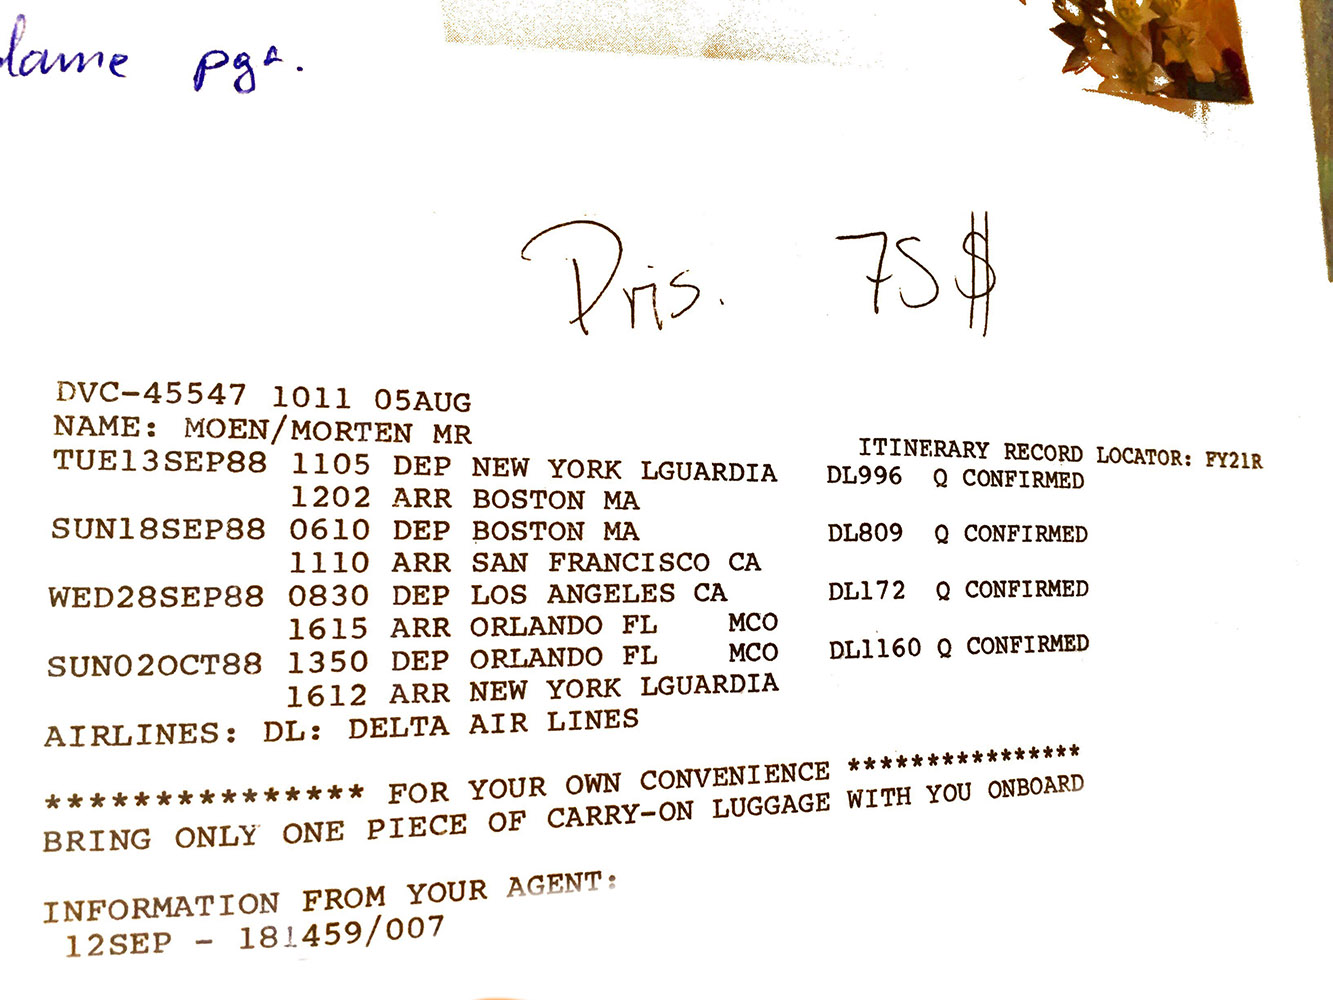
\includegraphics[width=200px]{images/tur-til-usa-1988/Flights.jpg}
	\caption{Også i 1988 kunne man få billige flyturer.}
\end{figure}

Så mandag 12. september fløy 17 studenter fra det som da var charter-terminalen på Gardermoen. Vi fløy med et flyselskap som het Tower Air. Dette var et charter-flyselskap som hadde startet opp i 1983 og som gikk konkurs i 2000. Dette selskapet kjøpte opp gamle fly fra andre selskaper og tilbød rimelige flybilletter. På sikkerhetsbeltene på vårt fly sto det klart og tydelig PanAm.

De hadde også et nokså uformelt crew. Vi kom ombord og satte oss, og en av oss gjorde det som mange gjør når de først finner plassen sin; han begynte å fikle med knappene i taket, men han klarte ikke å få på leselyset, så han tilkalte en flyvertinne. Eller flyvert, da. Dette eksemplaret av arten var en nokså kraftig mann, 2 meter høy med en ganske kraftig stemme. Vår venn forklarte at lys-knappen ikke fungerte. Denne nokså storvokste mannen bøyer seg over ham, prøver selv og har selvfølgelig ikke noen problemer med å få på lyset hvorpå han ser ned på vår nå nokså lille venn og sier “One more question, and you don’t eat”. Riktignok med et glimt i øyet, men vår venn spurte ikke om noe mer den turen.

I New York hadde vi bare en overnatting, på Royce Hotel rett ved LaGuardia-flyplassen, før vi fløy videre til Boston dagen etter. Ved frokosten på det hotellet lærte vi en viktig ting om USA. Vi møttes stort sett alle til frokost i restauranten. Frokost var ikke inkludert, så den ble betalt av hver enkelt. Etter som folk ble ferdige betalte de sin del og forlot restauranten. Det var først da de siste hadde betalt det som sto på sin regning og skulle til å gå at det smalt og vi ble klar over at tips IKKE er valgfritt i USA. Vi ble fulgt etter av rasende kelnere som forlangte å få det de skulle ha av tips. Så lærte vi det, liksom.

En kort flytur brakte oss til Boston som var et av hoved-stoppene på turen. Her sjekket vi inn på Best Western Homestead Inn litt utenfor sentrum. Her skulle vi bo i fem dager mens vi besøkte flere interessante bedrifter.

\begin{figure}
	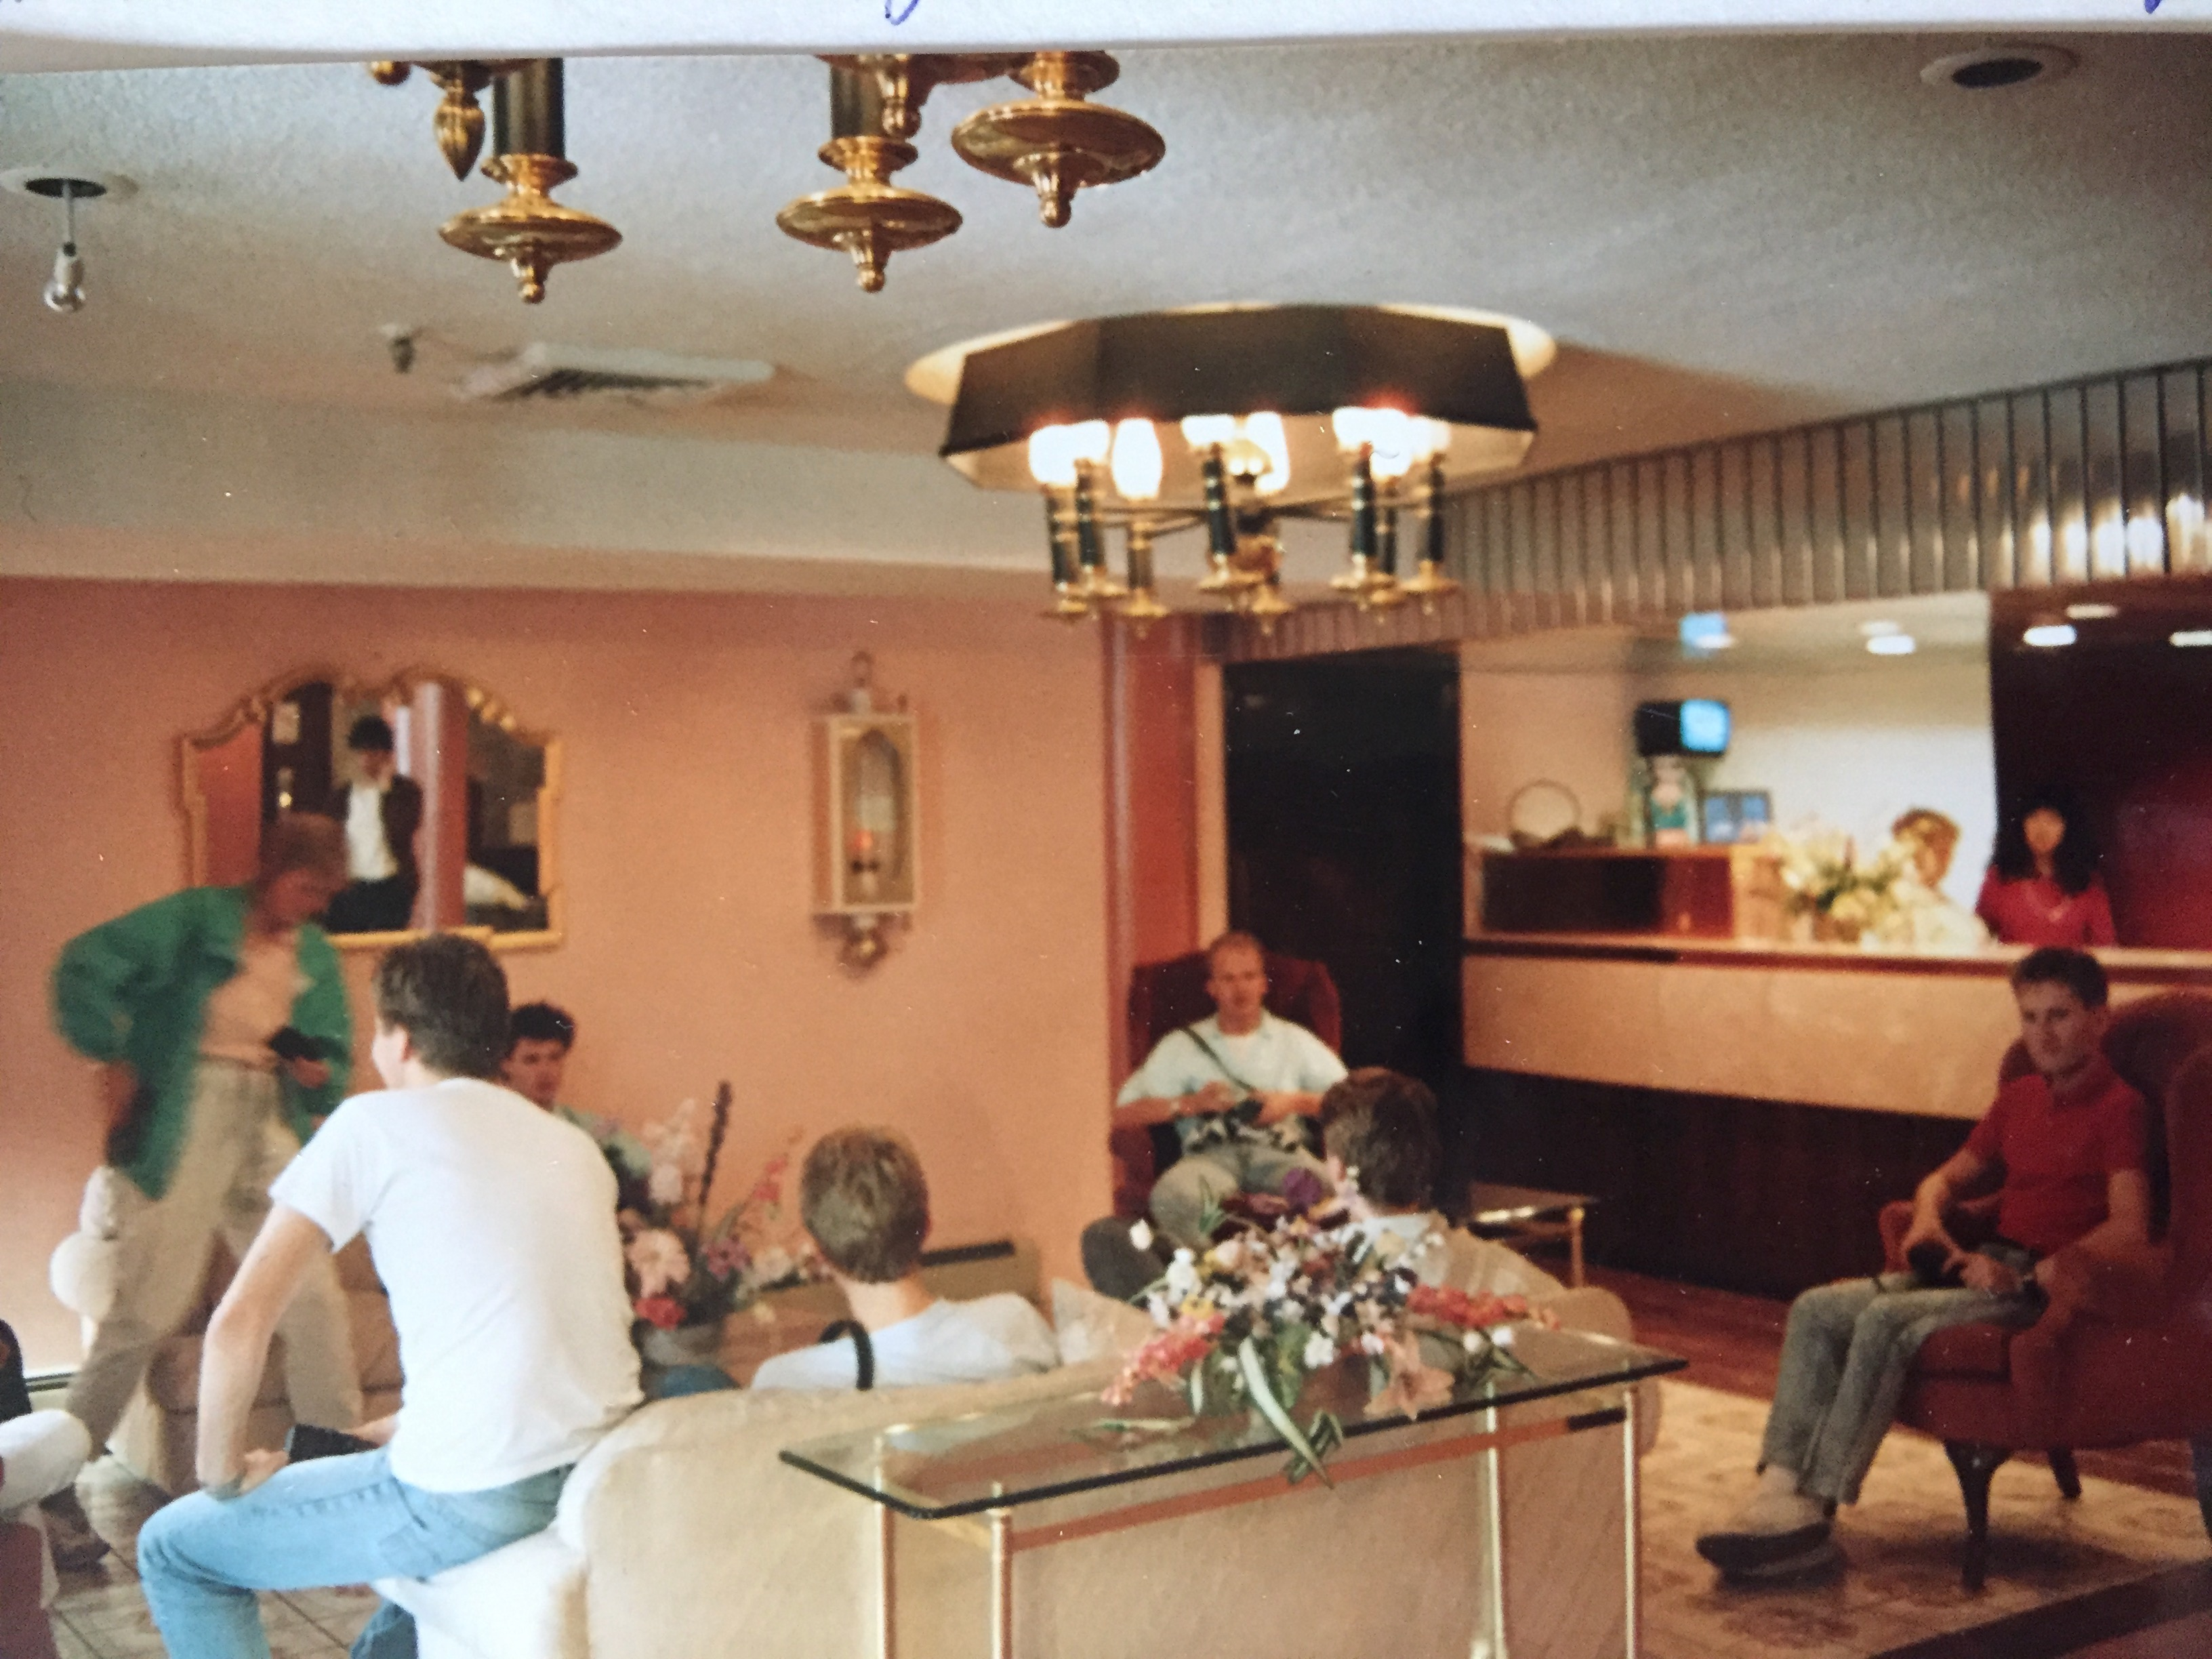
\includegraphics[width=\linewidth]{images/tur-til-usa-1988/IMG_3846.jpg}
	\caption{Fra resepsjonen på hotellet i Boston. Fra venstre: Anne Schiestad (i farta), ukjent (med ryggen til), Ole Christian Lingjærde, ukjent (med ryggen til), Geir Amdal, ukjent.}
\end{figure}

\section{Besøk hos Apollo Computer}

På 80-tallet var Apollo Computer et av de største navnene innen grafiske arbeidsstasjoner. I første halvdel av 80-årene var Apollo verdens største produsent av nettverks-arbeidsstasjoner og i 1986 ble firmaet også størst på “engineering workstations” med dobbelt så stor markedsandel som Sun som lå på andre plass.

\begin{figure}
	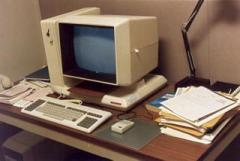
\includegraphics{images/tur-til-usa-1988/apollo_workstation.jpg}
	\caption{En Apollo arbeidsstasjon fra slutten av 80-tallet}
\end{figure}

Natten før Apollo-besøket skjedde det noe. Jeg (Morten) husker at jeg våknet av lyden av sikkerhetslenken på døren på hotellrommet. Noen hadde låst opp døren og forsøkt å komme inn, men ble stoppet av lenken. Jeg tenkte da at det kanskje var noen ansatte som prøvde å gå inn i feil rom eller noe slikt. Senere, da vi ble samlet til frokost skjønte jeg hva det var. I løpet av natten og morgentimene hadde det vært et innbruddsraid på hotellet.

Vi hadde stort sett tremanns-rom på hotellet, og på ett av våre rom hadde en av de tre gått ut, en sto på badet og en lå fortsatt og sov i sengen. Han på badet hørte døren gå opp og noen komme inn. Han trodde at det var romkameraten som hadde gått ut som kom inn igjen og gjorde seg ferdig på badet. Han som sov våknet ikke. Etter en kort stund gikk personen ut igjen, og da var i alle fall en klokke borte fra rommet.

Vi var ventet på Apollo tidlig på formiddagen, men på grunn av dette tyveriet måtte de som bodde på det ene rommet bli igjen for anmeldelse etc. Av en eller annen grunn følte flere at de også burde være igjen litt og hjelpe dem, så den første gruppen som kom frem til Apollo var relativt liten.

\begin{figure}
	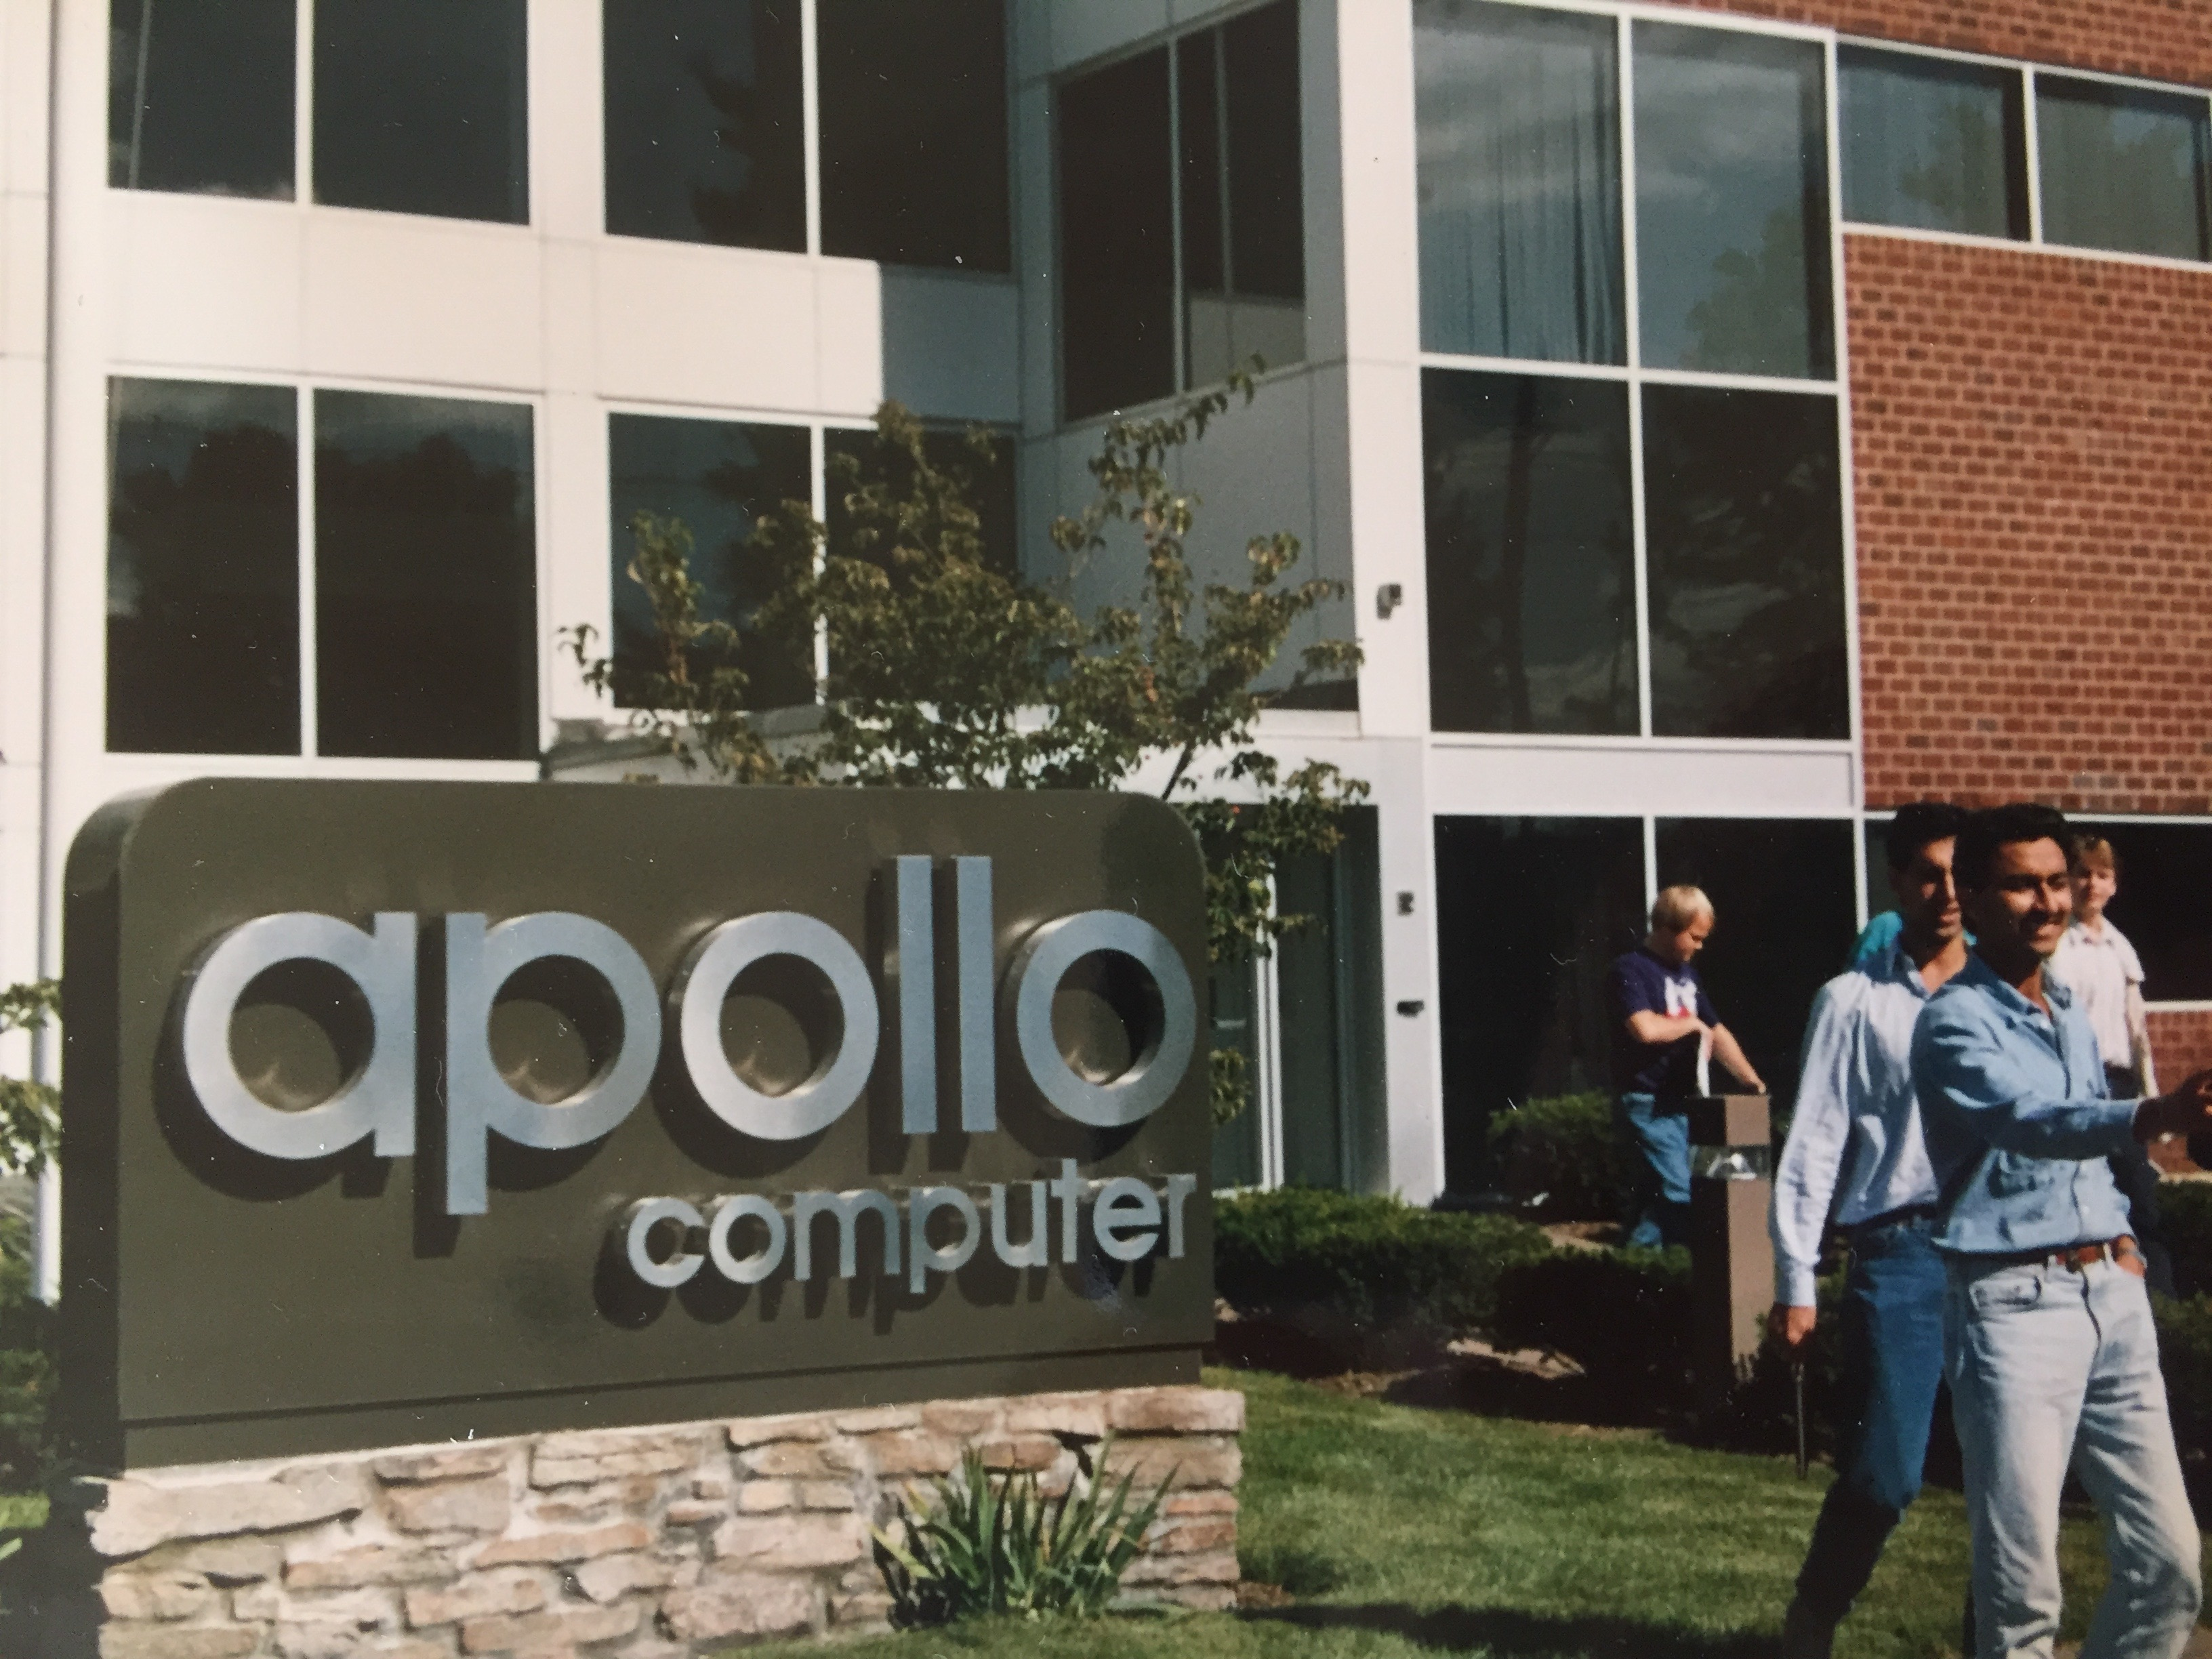
\includegraphics[width=\linewidth]{images/tur-til-usa-1988/IMG_3790.jpg}
	\caption{Noen av oss på vei ut fra Apollo Computers.}
\end{figure}

Apollo hadde imidlertid slått på stortromma og linet opp flere ledere inkludert Europa-sjefen i et møterom for oss for å fortelle om firmaet. Vi var vel en 4-5 mennesker som kom i den første puljen og prøvde oss på en slags forklaring om at vi hadde hatt innbrudd på et rom og at, eh … alle måtte være igjen på hotellet fordi en hadde fått klokken sin stjålet. Litt flaut. Resten av flokken kom frem en del forsinket og programmet kunne endelig starte.

Dette besøket viste en trend som vi opplevde på alle de stedene vi besøkte: Vi ble tatt veldig seriøst og vi ble veldig godt mottatt. Jevnt over ble vi møtt av høytstående mennesker som hadde lagt opp et stort og innholdsrikt program for oss.

Apollo begynte sin nedgang i slutten av 1987 og var altså på vei ned da vi var der. De ble kjøpt opp av HP i 1989 og mye av teknologien deres gikk inn i HPs 9000-serie av maskiner.

\section{Besøk hos Thinking Machines Corporation}

Et besøk som alle gledet seg til var Thinking Machines Corporation i Boston. Thinking Machines var egentlig en slags kuriositet og var et firma som laget en supercomputer som het Connection Machine. Firmaet ble startet i 1983 av Danny Hillis, og var basert på arbeid han gjorde i sin PhD-grad på MIT under veiledning av blant annet Marvin Minsky og Claude Shannon (førstnevnte var en av grunnleggerne av AI, mens sistnevnte var en av grunnleggerne av informasjonsteori).

\begin{figure}
	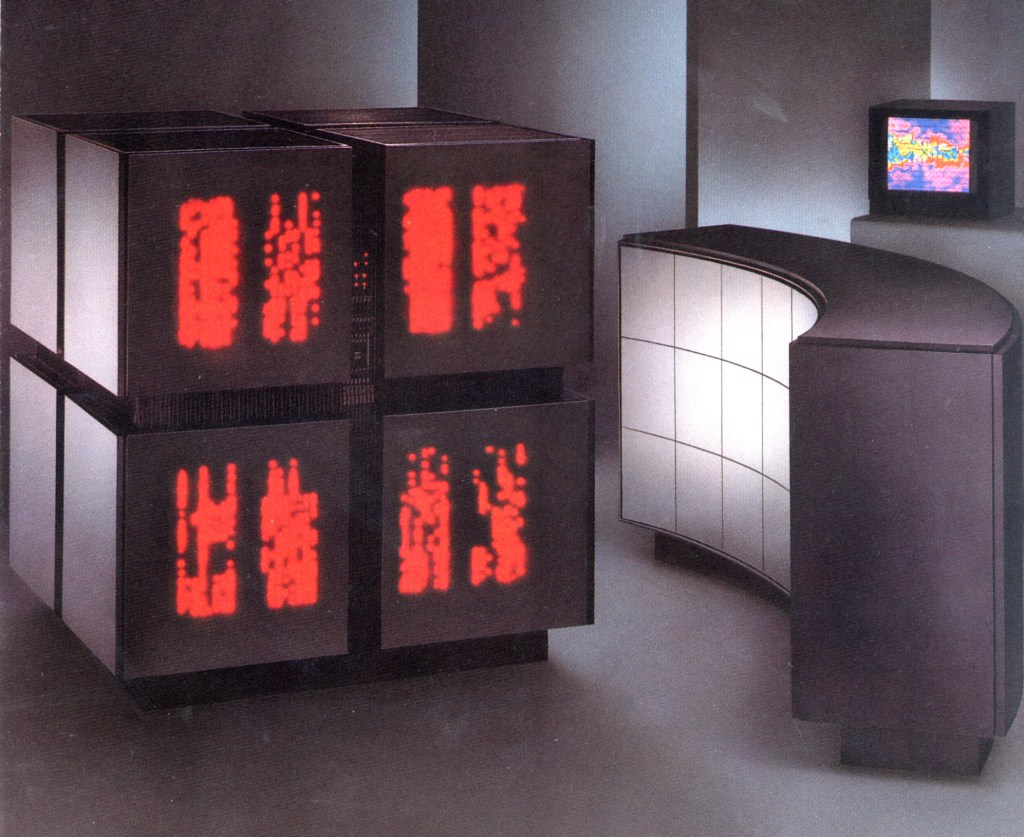
\includegraphics{images/tur-til-usa-1988/cm2.jpg}
	\caption{CM2 Connection Machine fra Thinking Machines Corp. inkludert det bardisk-formede disk-arrayet.}
\end{figure}

I 1993 var Connection Machine blant verdens raskeste datamaskiner. Connection Machine inneholdt svært mange prosessorer (CM-1 og CM-2 hadde over 64 000 prosessorer), der hver prosessor hadde direkte forbindelse til alle andre. Det er langt fra trivielt å utnytte så mange prosessorer på en effektiv måte, og både hardware og software i Connection Machine var nøye designet for å oppnå effektivitet. En av de som var involvert i dette arbeidet var den kjente fysikeren og Nobelpris-vinneren Richard Feynman. En morsom sak er at i filmen Jurassic Park som kom ut i 1993 kan vi se flere Connection Machines i parkens kontrollrom, og det er også flere henvisninger til firmaet og produktet andre steder i filmen. Maskinene var også seriøst kule å se på med et kubisk design med mengder av blinkene dioder og et array av harddisker som så mer ut som en bardisk enn noe annet. Bildet viser en CM-2 med 64 000 prosessorer og bardisk-formet disk-array. Firmaet gikk konkurs i 1994 og ble kjøpt av Sun Microsystems.

\section{Besøk på AI-laben på MIT}

MITs Artificial Intelligence Laboratory var kjent for å være et sted hvor store ideer ble født. Det var her mye av det tidlige fundamentet for forskningen på kunstig intelligens (AI) ble lagt. Programmeringsspråket LISP ble til her, og det var her Danny Hillis utviklet arkitekturen til Connection Machine som senere ble kommersialisert gjennom Thinking Machines Corporation (se eget avsnitt om besøket der). De fleste informatikere er også godt kjent med teksteditorene EMACS og GNUEMACS - disse ble begge utviklet av Richard Stallman nettopp på MIT AI-Lab. Vårt besøk på AI-laben fokuserte på deres robotforskning, og vi fikk se flere imponerende eksempler på roboter i aksjon da vi var der. Etter denne demo-runden hvor vi fikk svar på alle de spørsmål vi hadde, hørte vi et foredrag om AI-labens prosjekter. Vi hadde også på forhånd bedt om å få høre litt om hva de tenkte om fremtiden til nevrale nettverk, siden dette var et tema som på den tiden vakte stor interesse internasjonalt og som det var knyttet store forventninger til. Noe av grunnen til at vi ønsket å ta opp dette, var at det var en viss konkurranse mellom miljøene som jobbet med AI og miljøene som jobbet med nevrale nettverk på den tiden. Likevel kom det nokså uventet når vår vert på AI-laben - Carl Hewitt - fortalte at han knapt syntes nevrale nettverk var verdt å jobbe med. Han mente det kanskje var rom for to-tre mastergradsprosjekter på temaet, men ikke noe mer. En av grunnleggerne av AI-laben - Marvin Minsky - var også kjent for å ha et temmelig skeptisk syn på nevrale nettverk. Noen år senere døde interessen for nevrale nettverk nesten helt ut, mye på grunn av at de store forventningene ikke slo til. Noen få ildsjeler fortsatte imidlertid å studere dem, og for bare få år siden skjedde det et gjennombrudd i forskningen som ledet til det vi kaller “Deep Learning”. Deep Learning brukes i dag blant annet i Google Translate, i Apples Siri, til automatisk trading på New York børsen, og kan spille bedre poker enn profesjonelle pokerspillere. Om det er noe å lære av alt dette, så er det vel at det er vanskelig å spå mange år frem i tid når det gjelder teknologisk utvikling.

\section{Besøk på Computer Museum}

På den tiden var dette visstnok det eneste museet som i helhet var viet datafagets historie. Museet ga en lærerik og morsom innføring i både datamaskinens og programmeringens historie, og forsøkte seg også på noen fremtidsvisjoner. Det var mange hands-on demonstrasjoner, blant annet i bildebehandling, grafikk, bruk av roboter, kunstig intelligens og tale-gjenkjenning. I dag ville de fleste ha dratt kjensel på mange av disse anvendelsene fra sin egen mobiltelefon, men for 30 år siden var denne typen anvendelser langt fra dagliglivet og utrolig inspirerende å se og prøve.

\section{Logistikk}

Flyet fra Boston til San Francisco skulle gå kl 06:10. Det er ganske tidlig. Det var et stykke fra hotellet til flyplassen og vi trengte å finne en rimelig løsning.. Det ble nedsatt en komite (Morten og Ole Christian) for å ordne transporten. Løsningen ble at vi dro ut til flyplassen og leide en bil. Utifra det jeg kan se fra historieforskningen nå i etterkant må noen ha ordnet seg selv, for det var 13 stykker som skulle være med på dette stuntet. Vi satte opp en plan der første avgang gikk fra hotellet 02:30. Ole Christian var sjåfør på alle turene med fire passasjerer på hver tur. Neste tur gikk 03:30 og siste 04:30. klokken 05:00 var alle på flyplassen.

\begin{figure}
	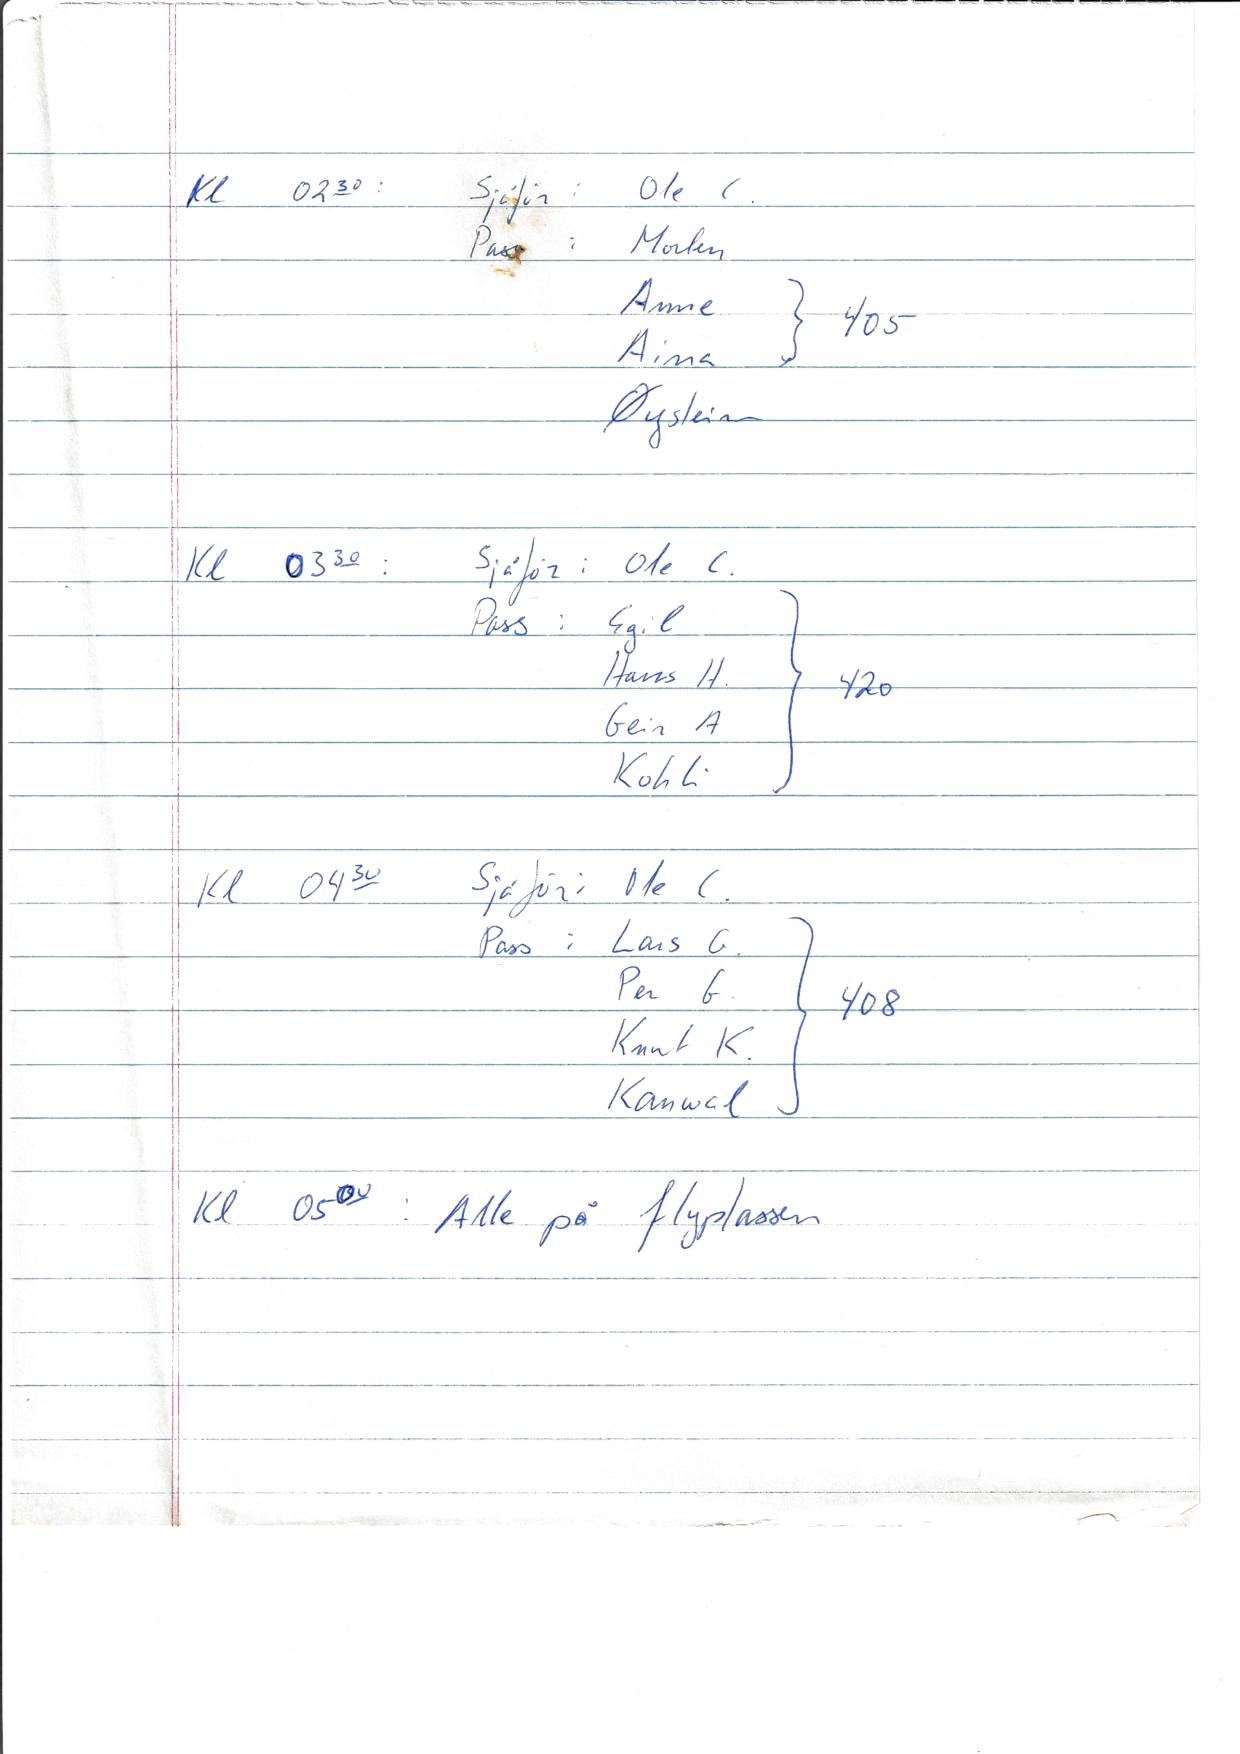
\includegraphics[width=200px]{images/tur-til-usa-1988/kjoring2.jpg}
	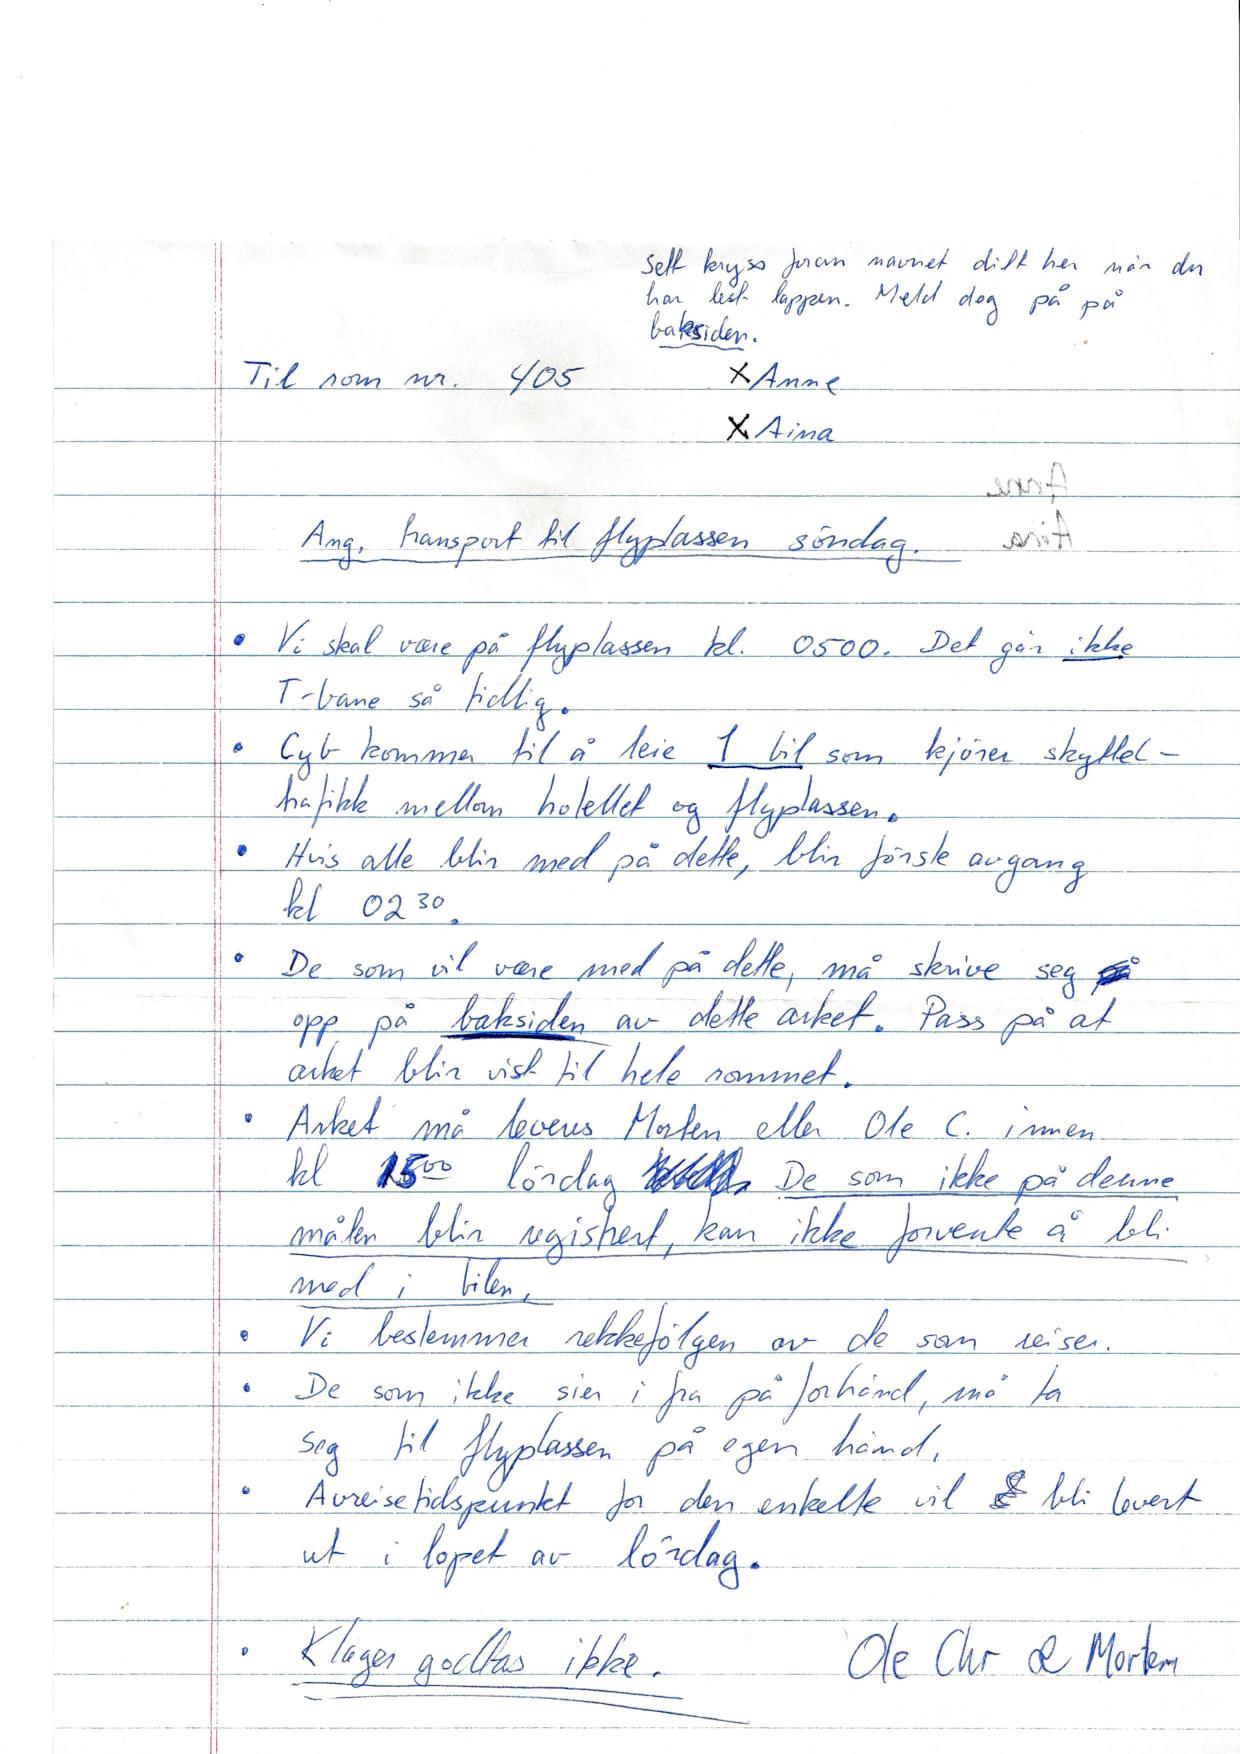
\includegraphics[width=200px]{images/tur-til-usa-1988/kjoring1.jpg}
\end{figure}

\section{San Francisco}

Etter mye faglig snacks i Boston fløy vi til San Francisco. Her hadde vi planlagt to besøk, ett hos Amdahl og ett hos Sun, men det ble også tid til sightseeing og nye opplevelser. For eksempel var den jalapenoen vi fikk på en mexikansk restaurant noe helt nytt for oss. Synd det ikke ble filmet.

\section{Amdahl Corporation og Sun Microsystems}

Generelt ble vi godt tatt imot hos alle de firmaene vi var på besøk hos, men Amdahl overgikk de andre. De hadde booket konferanserom på et førsteklasses hotell og stilte med så mye sjefer at man skulle tro de forventet ledelsen fra UiO og ikke en bunke med studenter. De serverte oss også en ganske så voldsom lunch.

\begin{figure}
	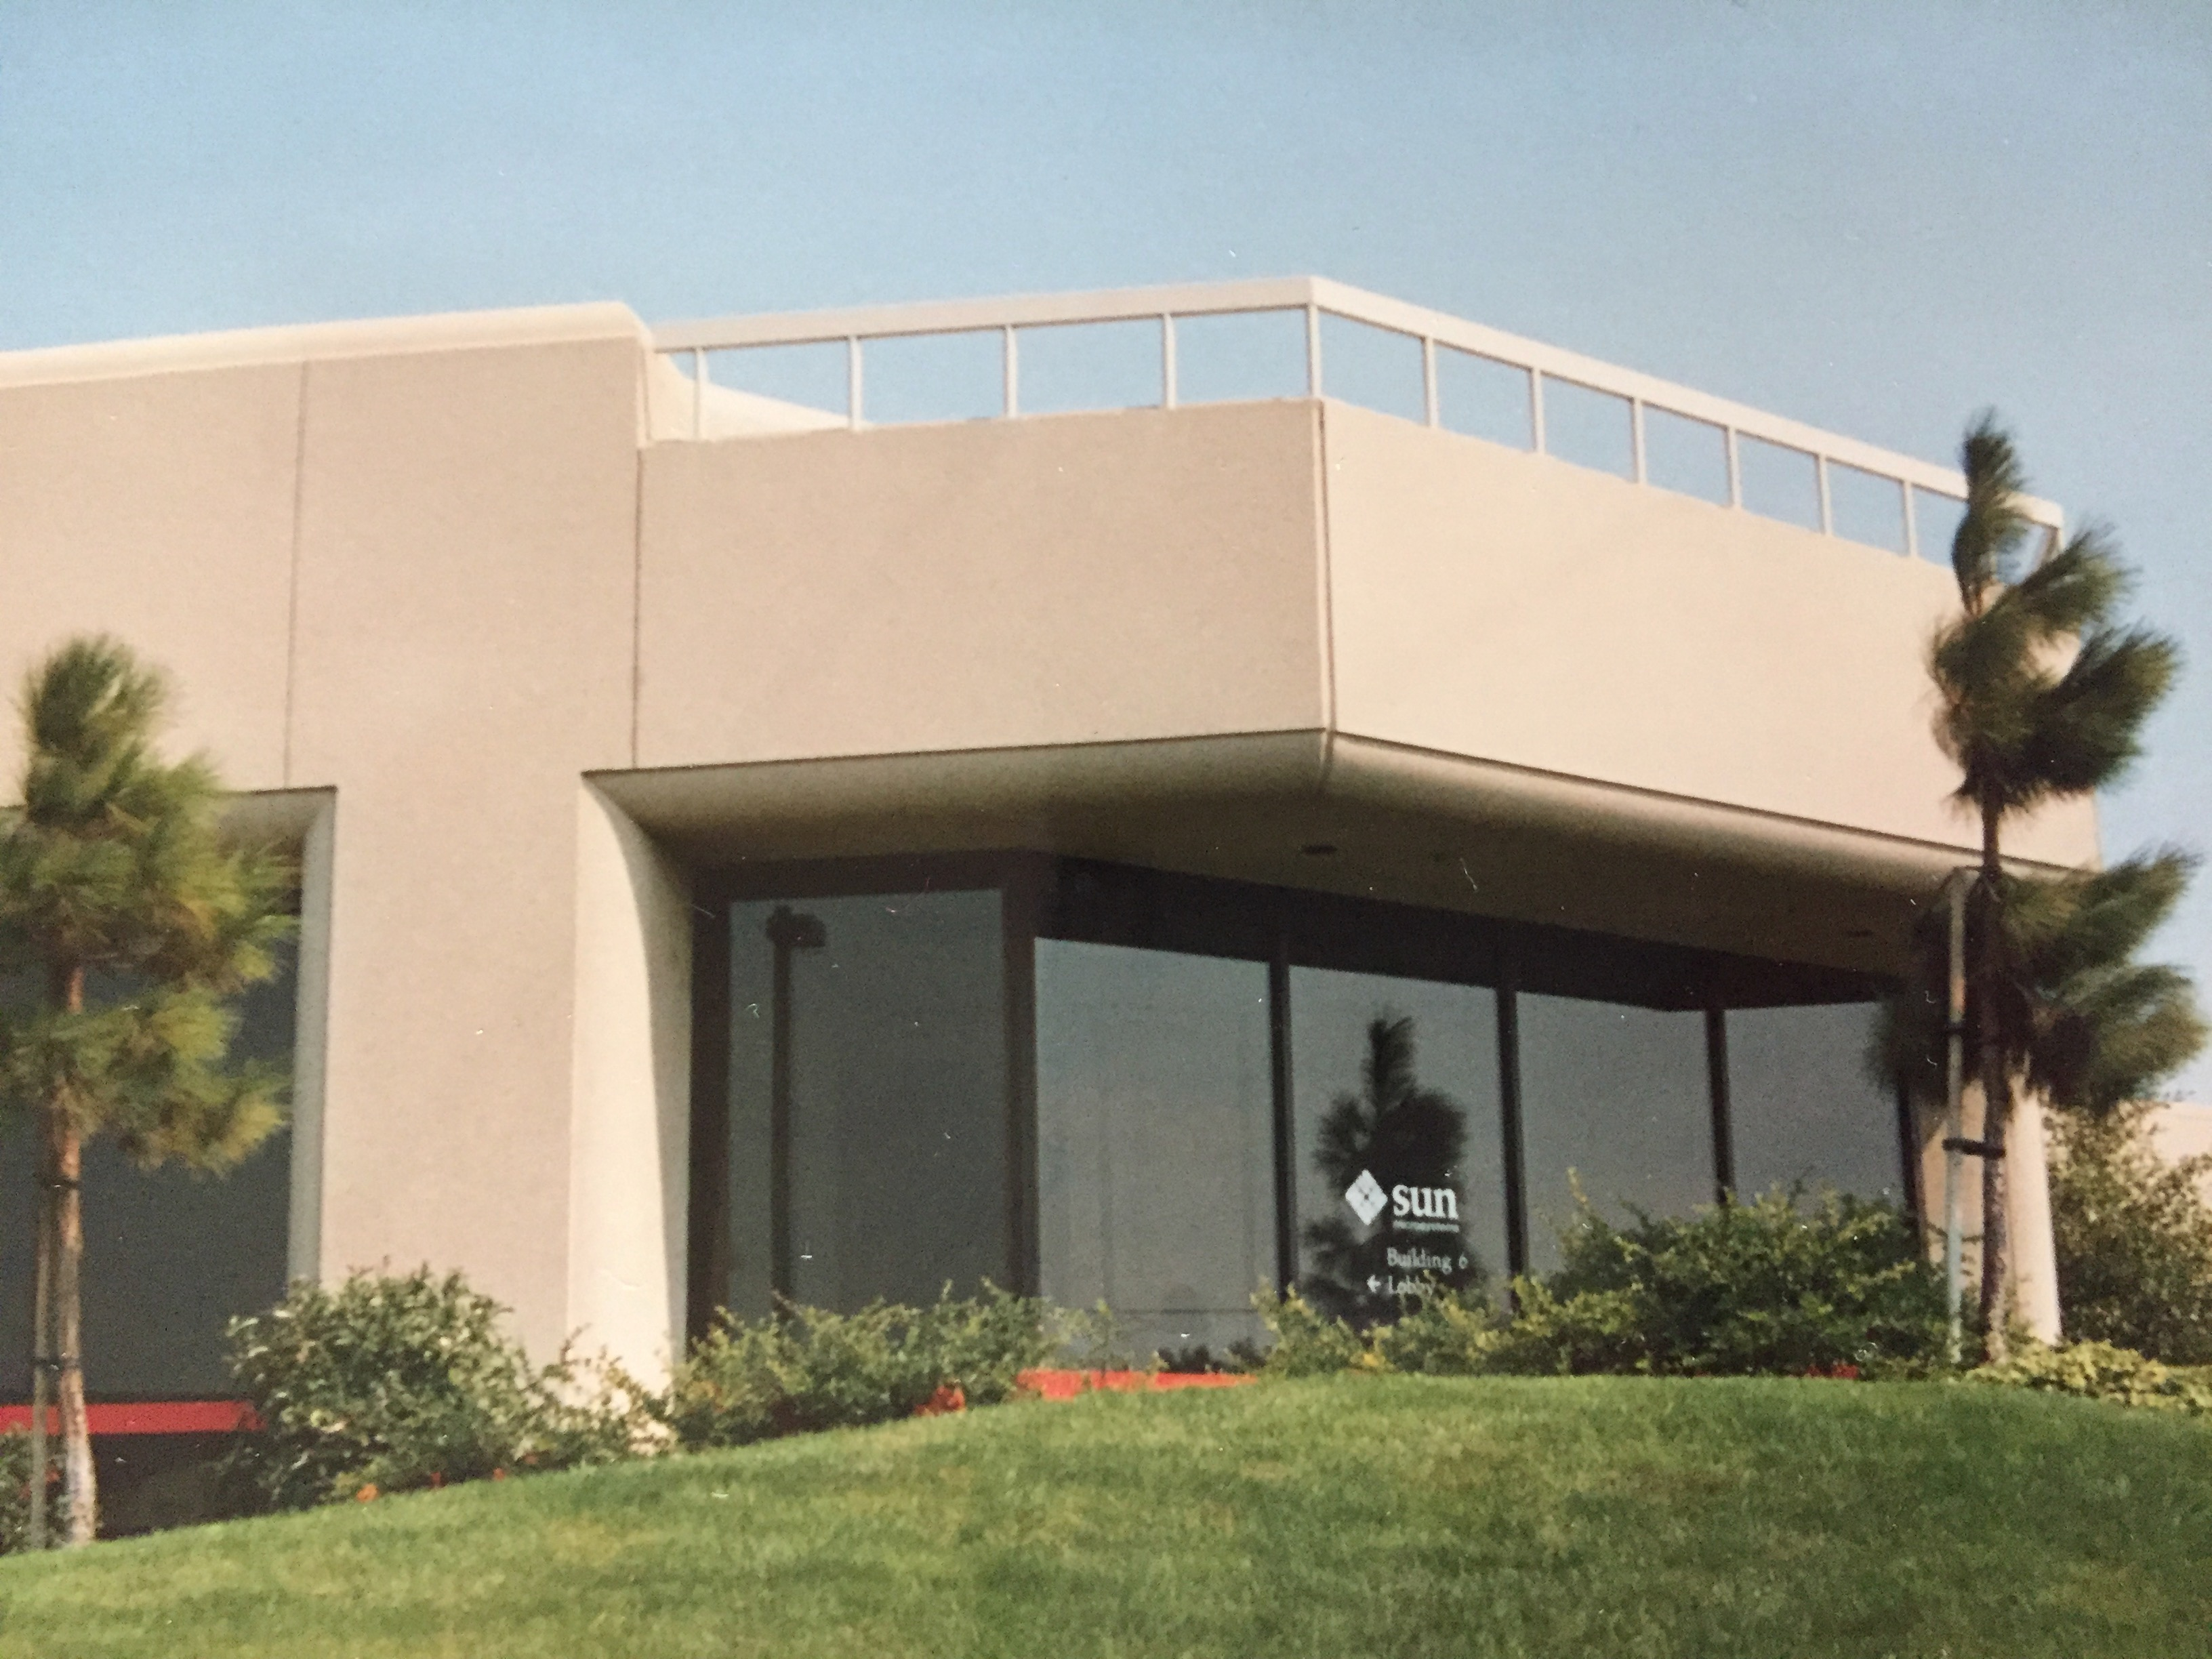
\includegraphics[width=\linewidth]{images/tur-til-usa-1988/IMG_3847.jpg}
	\caption{Sun Microsystems, Silicon Valley.}
\end{figure}

Også Sun tok vel imot oss. Et av temaene der var grafiske brukergrensesnitt der Suns arbeidsstasjoner lå langt fremme. Sun ble startet i 1982 av Vinod Khosla, Andy Bechtolsheim og Scott McNealyog som alle var studenter ved Stanford og de hadde hovedkvarter i Santa Clara i Silicon Valley. De ble fort en av de ledende innen grafiske arbeidsstasjoner og var også en av de ledende innen utviklingen av Unix. Det som Sun nå kanskje er mest kjent for er at de utviklet programmeringsspråket Java.

I år 2000 begynte det å gå nedover med firmaet og de ble overtatt av Oracle i 2008.

\section{Avslutning}

Etter Amdahl og Sun var det faglige over. Fra San Francisco delte vi oss i grupper som leide biler og kjørte ned til Los Angeles og tilbrakte noen dager der. Noen av oss kjørte Highway One nedover langs kysten. Morten kjørte med Øystein, Hans Henrik og Geir i en Lincoln Town Car som de var rimelig stolte over.

\begin{figure}
	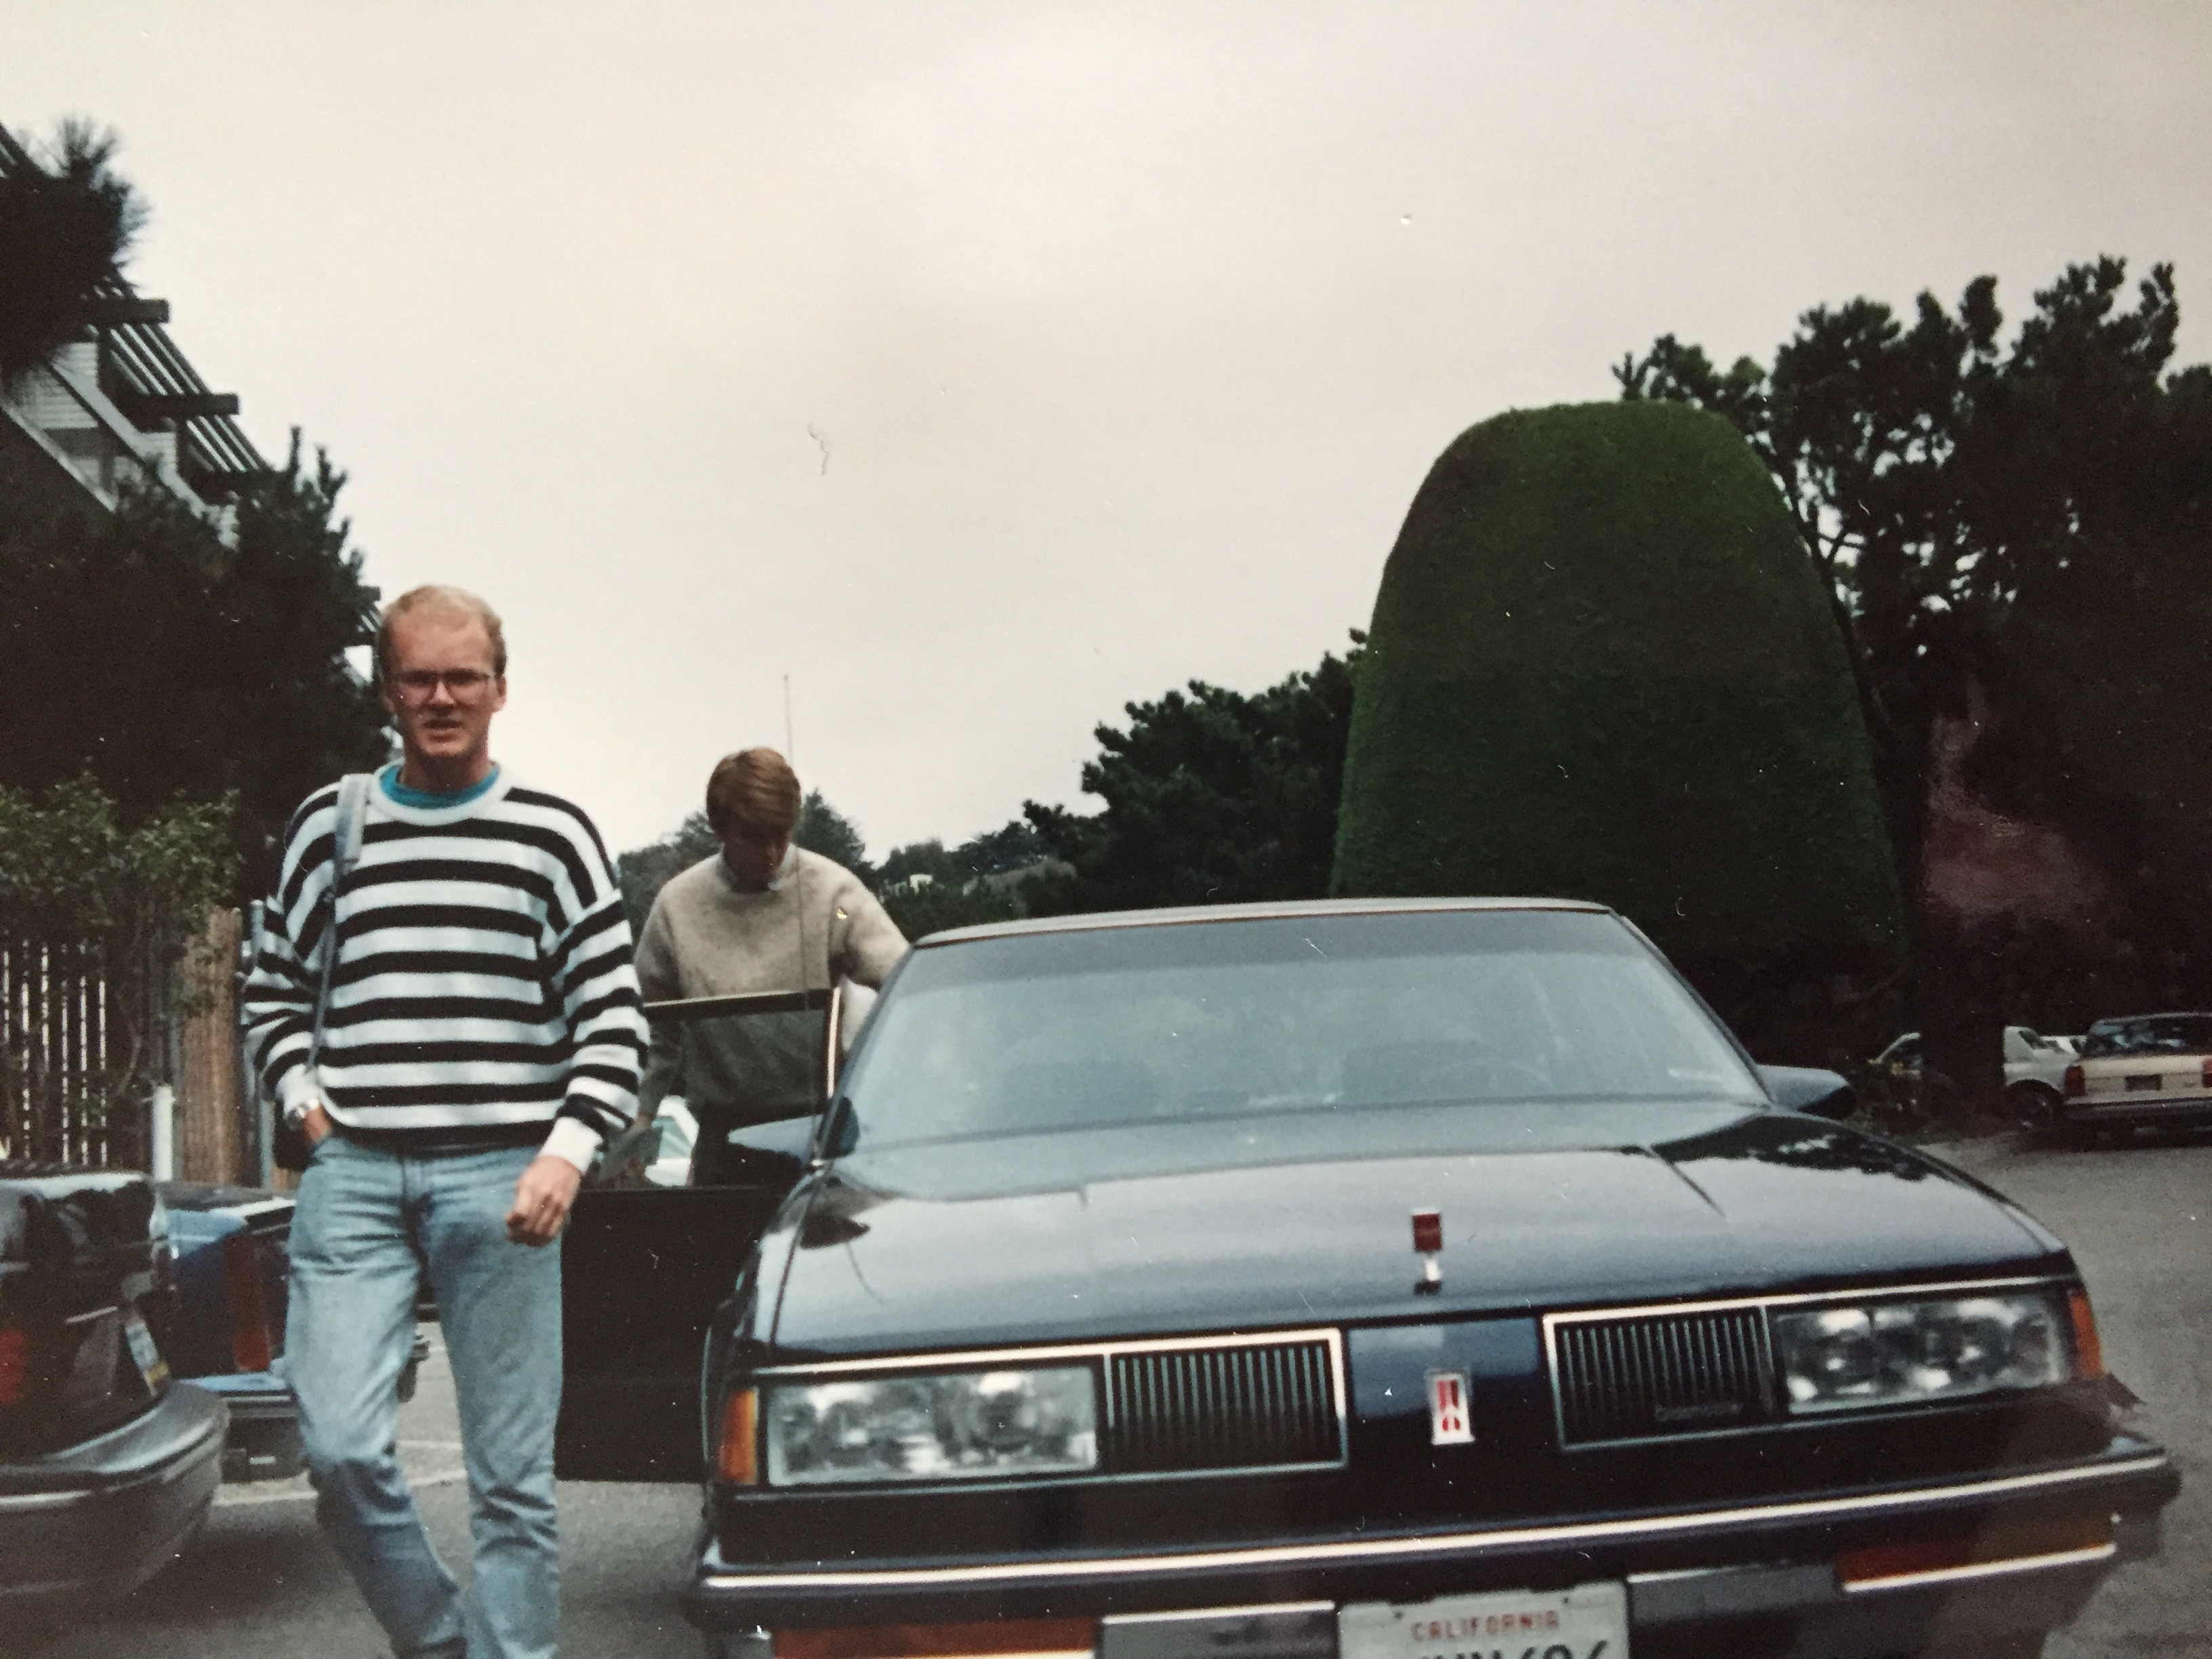
\includegraphics[width=\linewidth]{images/tur-til-usa-1988/IMG_3848.jpg}
	\caption{Stolte av leiebilen, en Lincoln Town Car, fra venstre: Geir Amdal, Hans Henrik Eriksen.}
\end{figure}

Denne gruppen overnattet i Santa Barbara på vei ned, og der traff de crewet fra en av de andre bilene.

\begin{figure}
	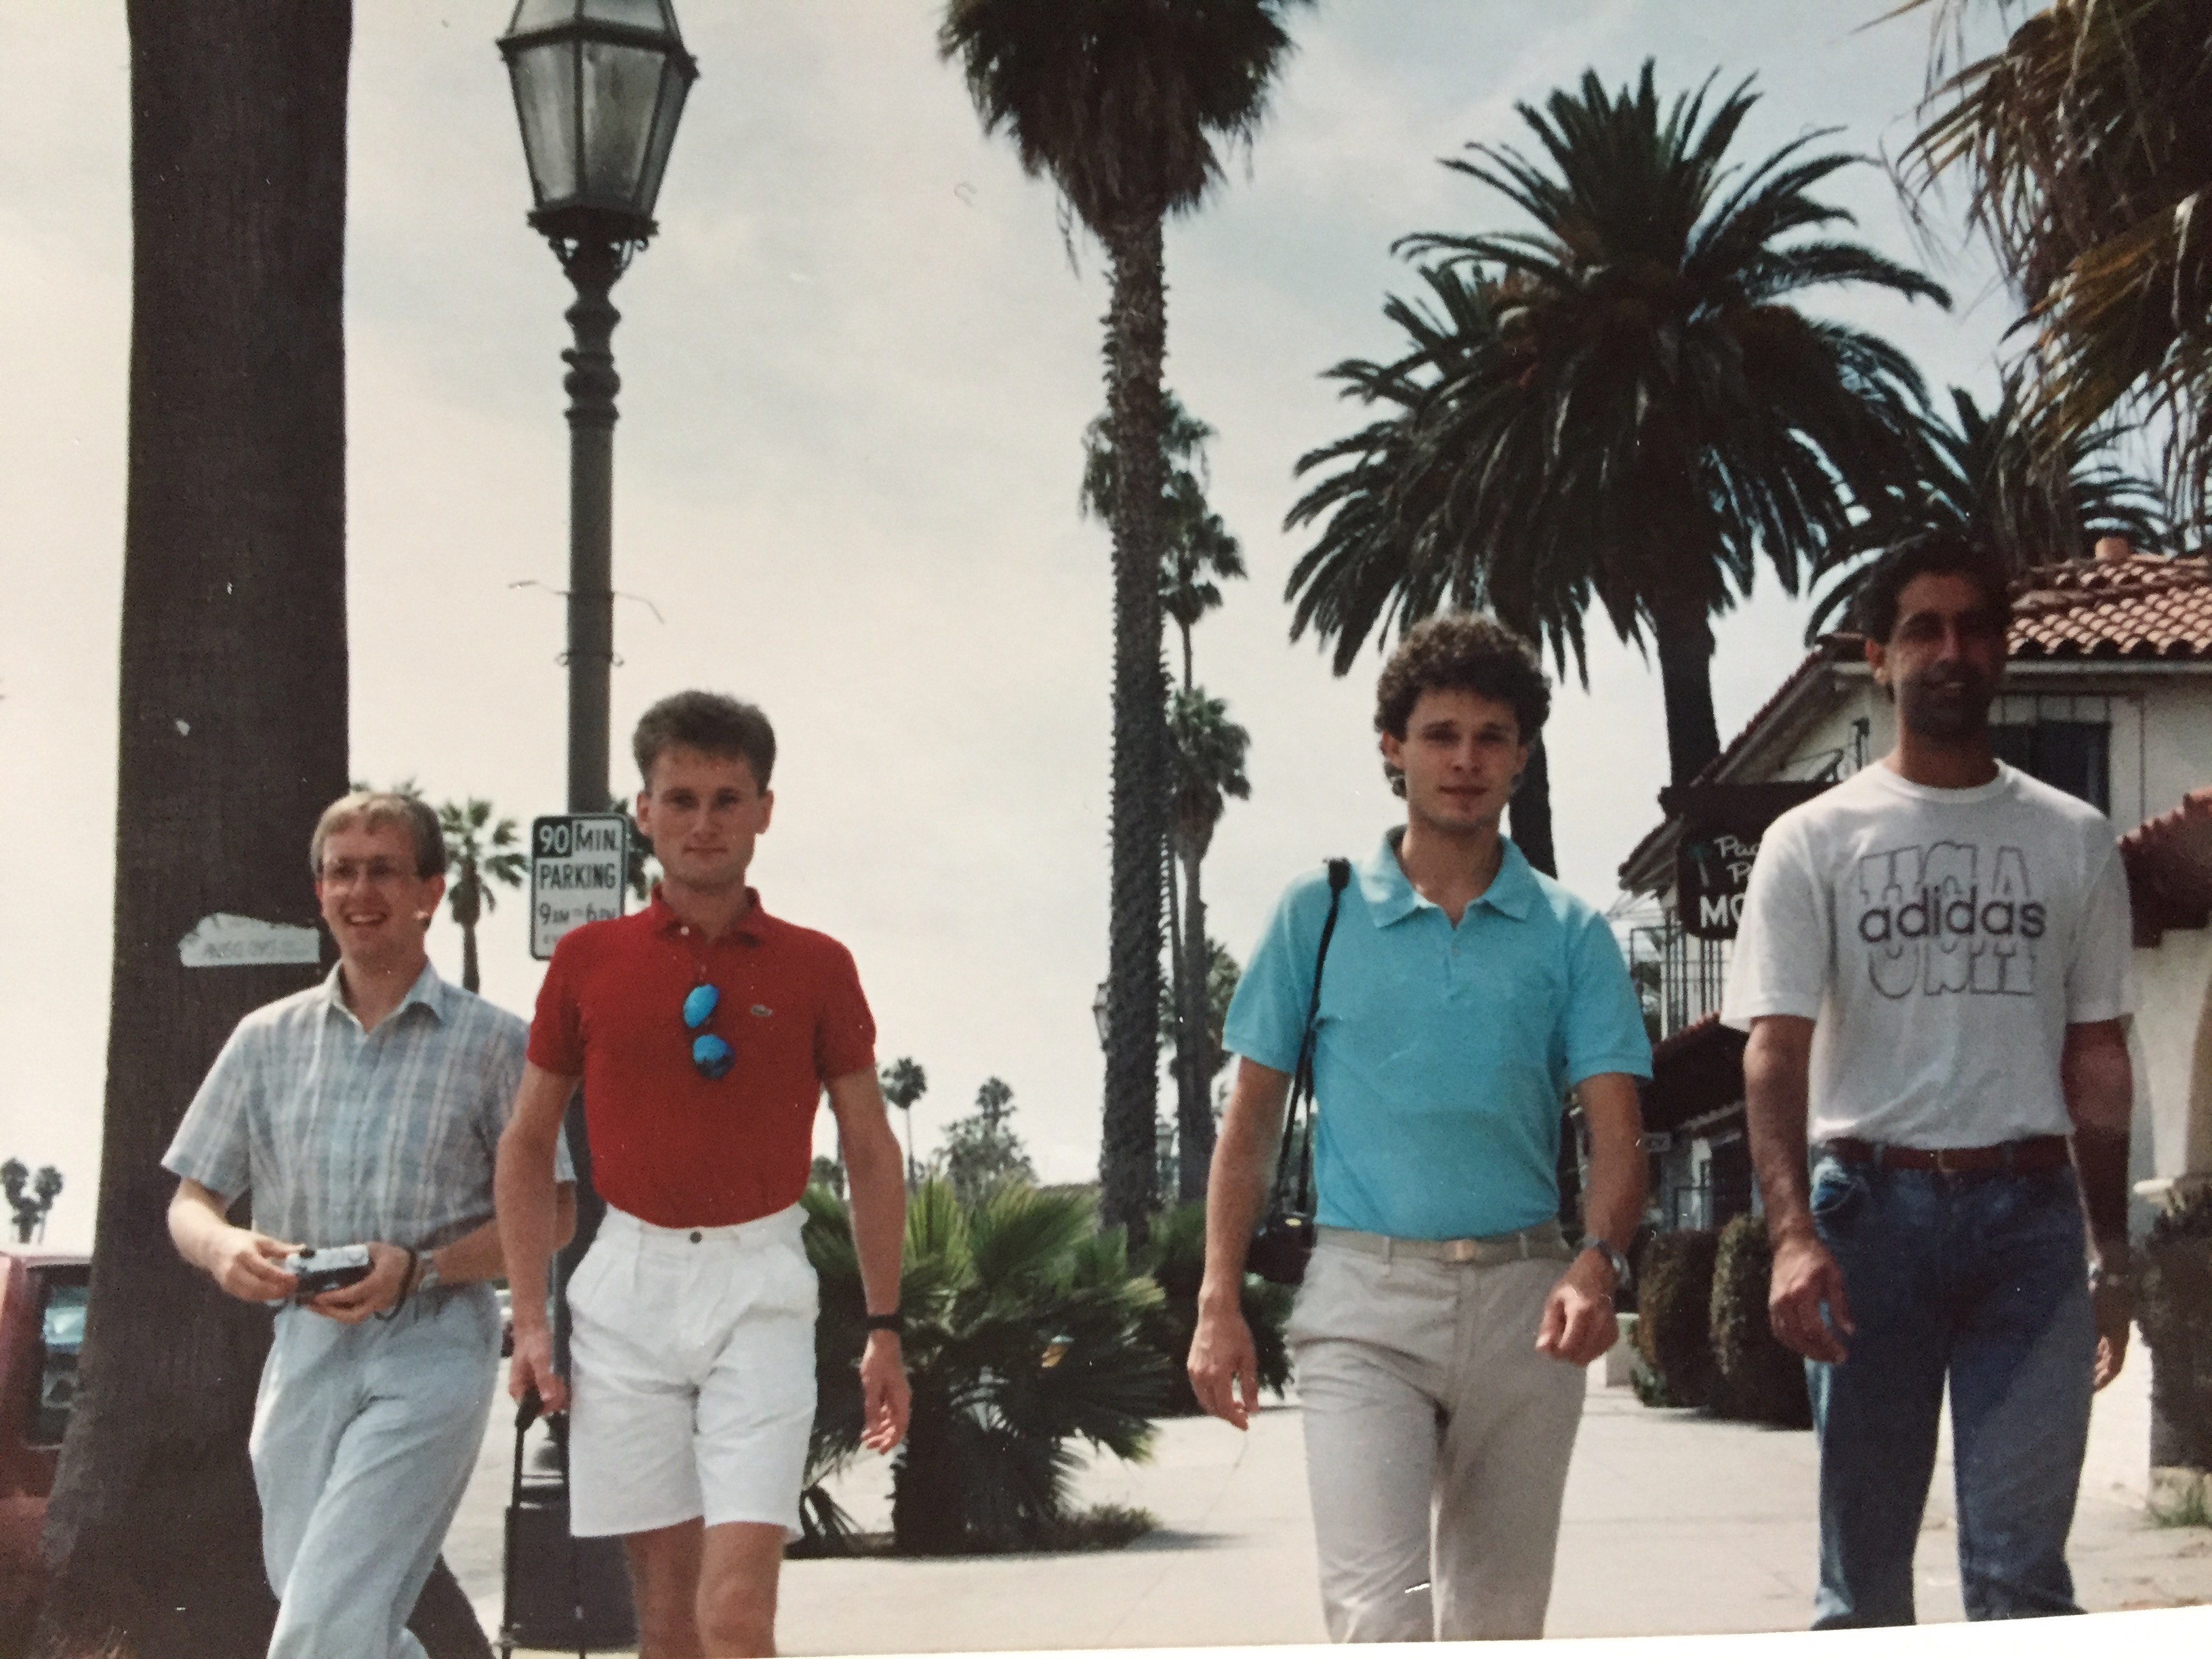
\includegraphics[width=\linewidth]{images/tur-til-usa-1988/IMG_3849.jpg}
	\caption{I Santa Barbara, fra venstre: Anders Ellefsrud, ukjent, Ole Christian Lingjærde, ukjent.}
\end{figure}

Etter noen dager i Los Angeles med sightseeing, Hollywood og Universal Studios fløy vi videre til Orlando i Florida. Her ble vi noen dager og fikk testet litt soling og bading. Vi fikk også tatt turen innom Disney World og Epcot.

\begin{figure}
	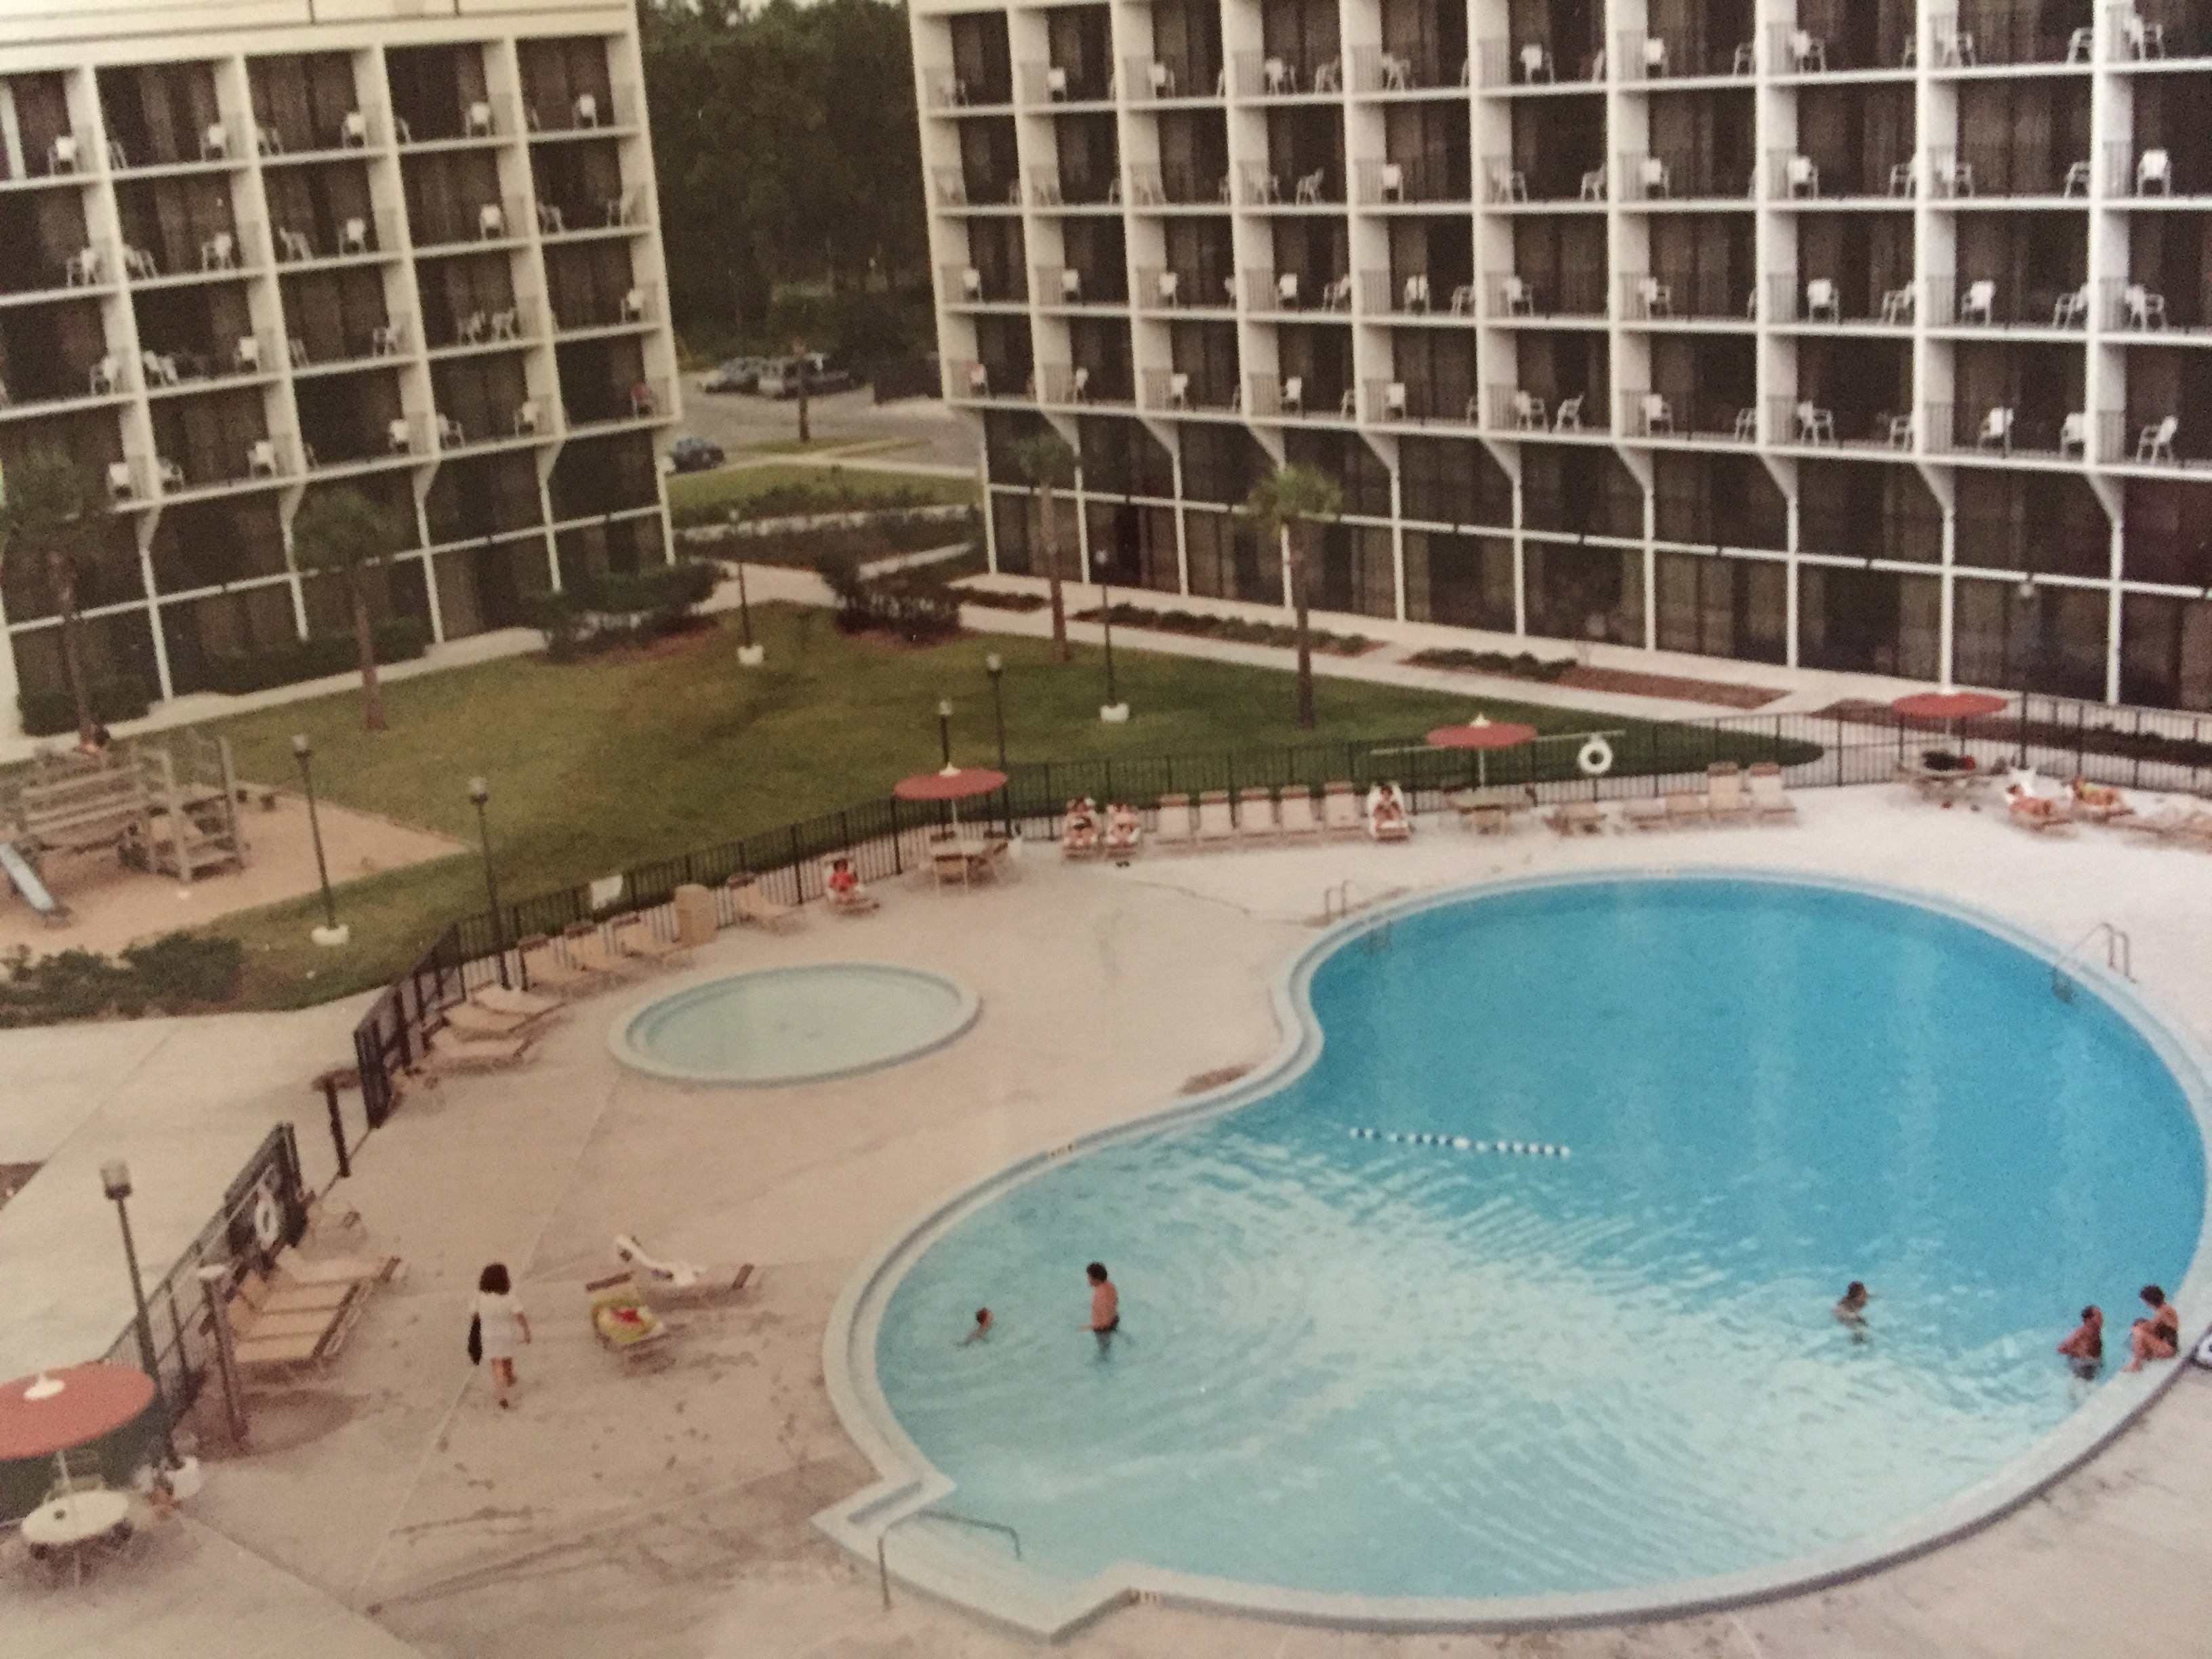
\includegraphics[width=\linewidth]{images/tur-til-usa-1988/IMG_3852.jpg}
	\caption{Fra hotellet i Orlando}
\end{figure}

Noen fikk også tid til en tur til Kennedy Space Center. Dette var det året den første romfergen etter den som eksploderte ble skutt opp, og det skjedde faktisk mens vi var i Orlando og mye handlet om akkurat det. Man kunne kjøpe (og kjøpte) en mengde romferge-relaterte ting som frysetørret astronaut-is og The Space Shuttle Operator’s Manual.

\begin{figure}
	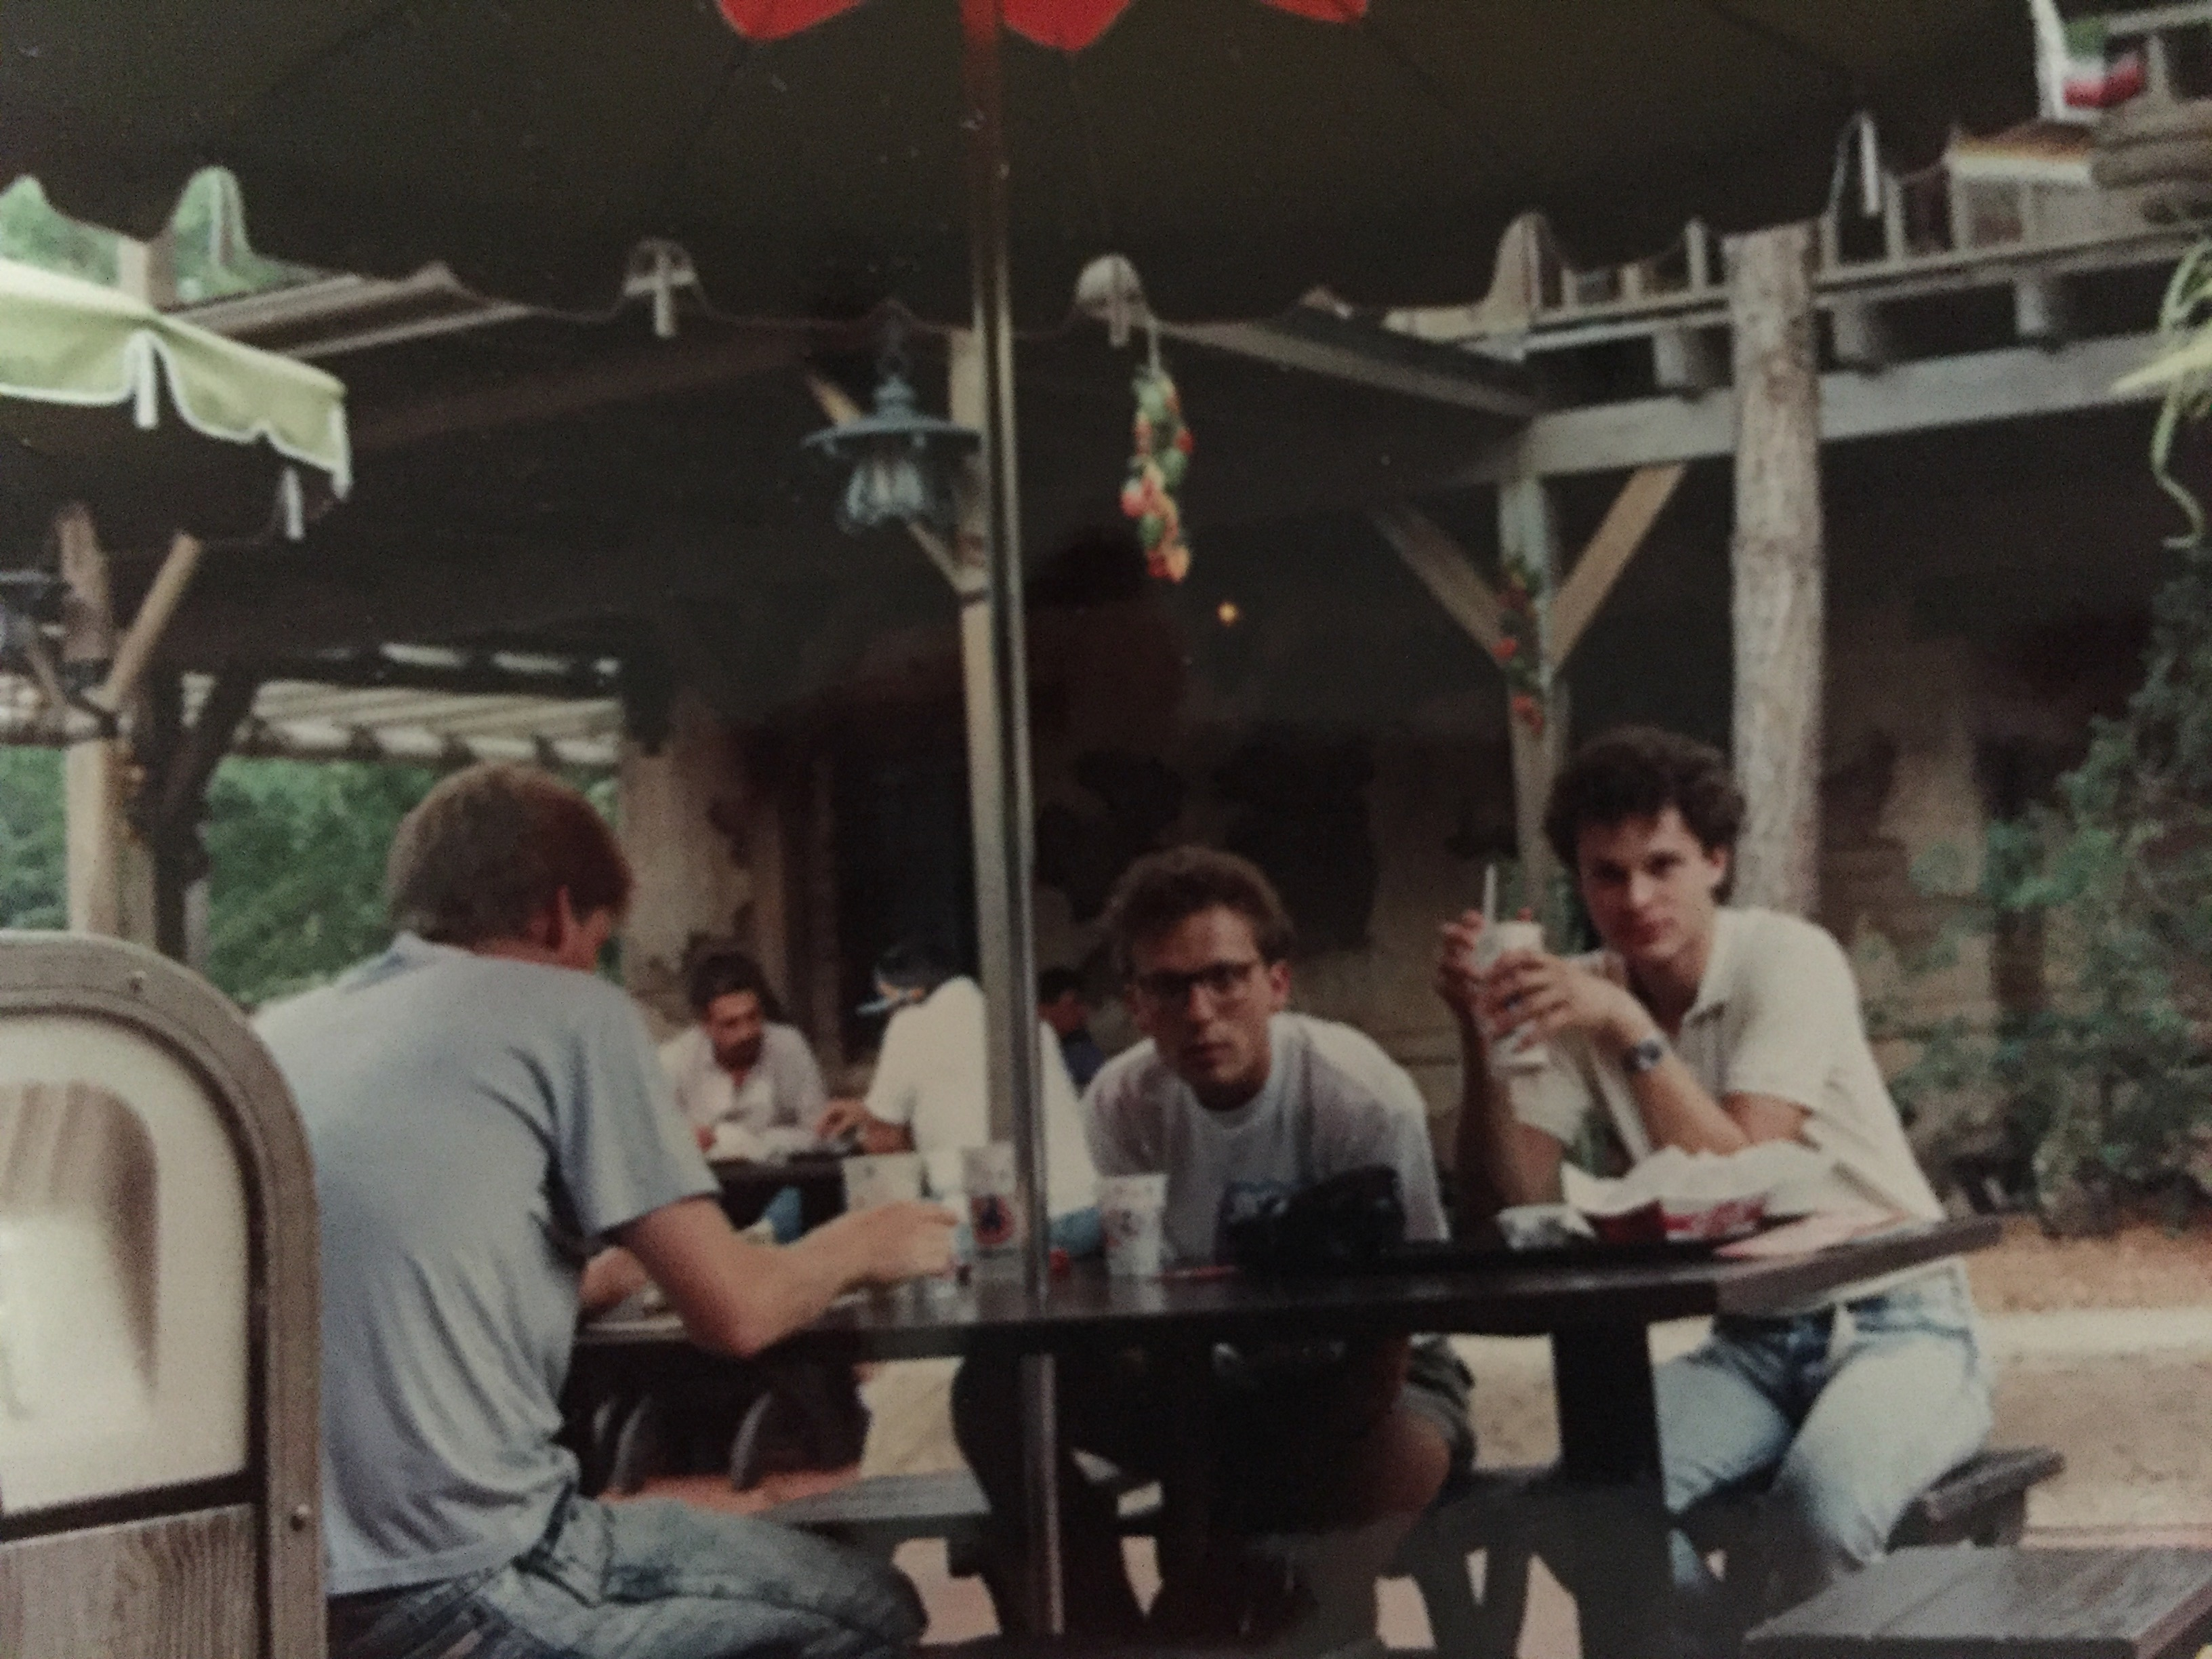
\includegraphics[width=\linewidth]{images/tur-til-usa-1988/IMG_3850.jpg}
	\caption{Man får seg litt mat i Disney World, fra venstre: ukjent, Øystein Wolff, Ole Christian Lingjærde.}
\end{figure}

Da romfergen ble skutt opp var noen av oss i Disney World. Jeg (Morten) husker Ole Christian og jeg kom ut fra en bygning der vi hadde sett noen gamle Mikke-filmer og la merke til at alle sto og så opp. Vi kikket også opp, og der var romfergen på vei opp.

Etter noen dager i Florida fløy vi tilbake til New York og hjem.

Vi tror at de fleste som var med på turen husker den som et av høydepunktene i studietiden. Vi fikk sett en del av USA, opplevde mye og fikk besøke noen av verdens største og mest innovative firmaer. Noe som man kan tenke over i ettertid er at bortsett kanskje fra MIT, Apollo som fortsatt kan ha noe arvegods i HP og at noe av Sun kan finnes hos Oracle er alle disse firmaene nå borte…

\begin{figure}
	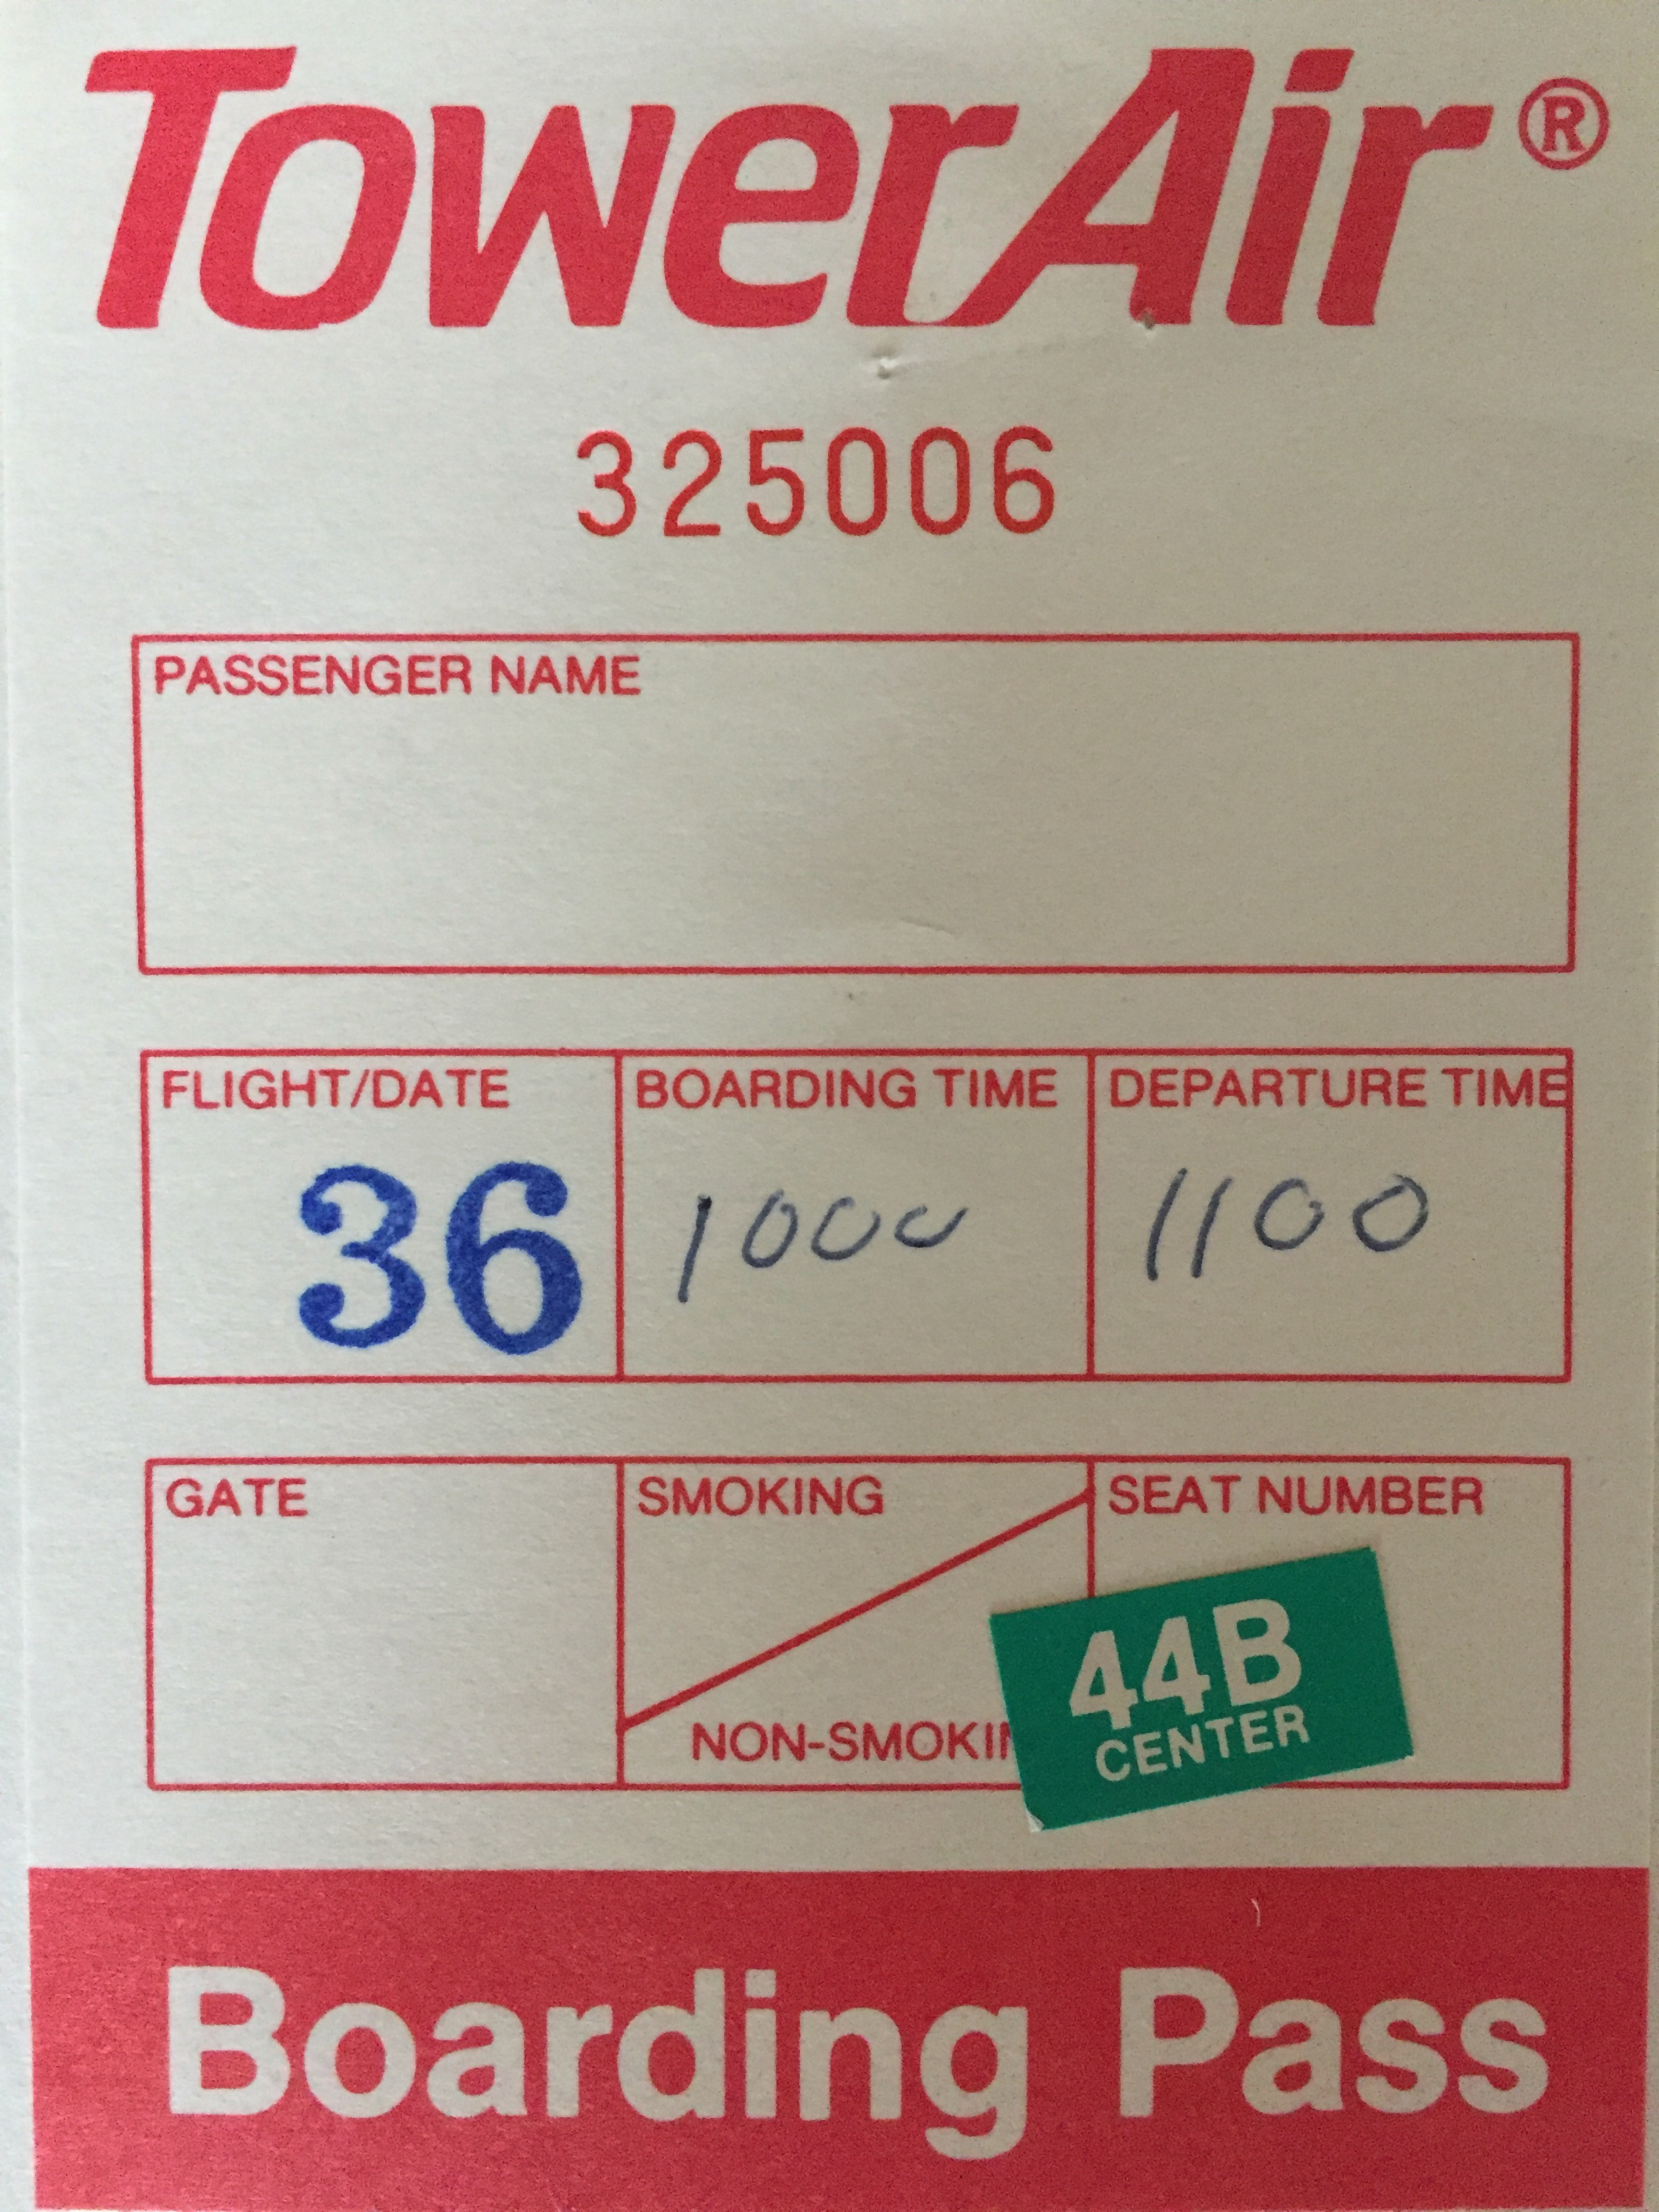
\includegraphics[width=\linewidth]{images/tur-til-usa-1988/IMG_3853.jpg}
\end{figure}
